\documentclass[11pt,a4paper,openright]{report}
\usepackage{float}
\usepackage{amsmath}
\usepackage{booktabs}
\usepackage{graphicx}
\usepackage{listings}
\usepackage{graphicx}
\usepackage{pst-rel-points}
\usepackage{pstricks}
\usepackage{pst-node}
\usepackage{pst-text}
\usepackage{auto-pst-pdf}
\usepackage{etex}
\usepackage{verbatim}
\usepackage{pgfplots} 
\usepackage{courier}
\lstset{basicstyle=\footnotesize\ttfamily}

\pgfplotsset{width=10cm,compat=1.5}
\restylefloat{table}
%\usepackage{ps2pdf}

%%\lstset{language=C}
\title{\textbf{M. Tech Project Stage-II Report}\\ on \\\textbf{Incremental Data flow Analysis using PRISM}}
\vspace{2.5cm}
\author{\emph{by}\\ \\ \bf{Rashmi Rekha Mech}\\\bf{Roll No : 133050089} \\
\\ \emph{Under the Guidance of}\\ \\\textbf{Prof. Uday Khedker}\\}
\date{}


\begin{document}

\maketitle
%\begin{comment}
\begin{abstract}

When a program undergoes changes during development, updating the data flow information by doing exhaustive analysis is very cost 
inefficient. So incremental data flow analysis is used which modifies only those data flow information of a program that has
been changed, rather than recomputing entire data flow information of a program. The incremental analysis methods are known for bit-vector framework.
These methods are not directly applicable to constant propagation. This report presents some issues in doing incremental analysis in Constant Propagation.

This report also discribes PRISM, an analyzer generator developed at Tata Research Development and Design Centre (TRDDC). We plan to enhance PRISM to support 
incremental data flow analysis.

\end{abstract}
%\end{comment}

\tableofcontents

\listoftables

\listoffigures

\cleardoublepage
\setcounter{page}{1}
\pagenumbering{arabic}
%%%%%%%%%%%%%%%%%%%%%%%%%%%%%%%%%%%%%%%%%%%%%%%%%%%%%%%%%%%%%%%%%%%%%%%%%%%%%
\chapter{Overview}
\section{Introduction}
When a program undergoes changes during development, some or all of data flow information computed earlier becomes invalid.
Thus, recomputation of data flow values is required.
\subsubsection{Motivating Example}
Consider a control flow graph in Fig~\ref{fig:Intro_ex}~\cite{thesis_r} for available expression analysis. Table~\ref{tab:Initial Available_exp}(a) shows 
an initial result which requires three iterations to converge. Suppose, expression $a+b$ in node $n6$ has been removed. To reflect this change, recomputing
data flow information from scratch is shown in Table~\ref{tab:Initial Available_exp}(b). 

The removal of expression $a+b$ does not affect the data flow values and hence no new information is added as shown in Table~\ref{tab:Initial Available_exp}(b).
For such changes, it is not desirable to recompute the information from scratch. This may unnecessarily analyze unaffected program behaviours which 
leads to redundant computation of old values which is very inefficient. 

For such changes, incremental data flow analysis can be used. It modifies only those data flow information which has been affected by 
the change rather than recomputing entire data flow information. It is more cost-effective than an exhaustive analysis.



\begin{figure}[H]
\centering
\psset{unit=1mm}
\begin{pspicture}(0,0)(100,90)
% \psframe(0,0)(100,90)
\putnode{n1}{origin}{50}{80}{%
     \psframebox[linewidth=.3,framesep=1.5]{\begin{tabular}{c} $a*b$ \\ $b+d$
                                             
                                            \end{tabular}
}}
\rput(35,80){\rnode{a}{n1}}
\putnode{n2}{n1}{0}{-15}{%
     \psframebox[linewidth=.3,framesep=1.5]{$a+b$}}
\rput(40,65){\rnode{a}{n2}}
\putnode{n3}{n2}{-20}{-15}{%
     \psframebox[linewidth=.3,framesep=1.5]{$b+d$}}
\rput(20,50){\rnode{a}{n3}}
\putnode{n4}{n3}{0}{-15}{%
     \psframebox[linewidth=.3,framesep=1.5]{\begin{tabular}{c} $a=1$ \\ $a+b$
                                             \end{tabular}
}}
\rput(15,35){\rnode{a}{n4}}
\putnode{n5}{n2}{20}{-30}{%
     \psframebox[linewidth=.3,framesep=1.5]{$d=1$}}
\rput(60,35){\rnode{a}{n5}}
\putnode{n6}{n5}{0}{-15}{%
     \psframebox[linewidth=.3,framesep=1.5]{$a+b$}}
\rput(60,20){\rnode{a}{n6}}

\putnode{n7}{n6}{0}{-15}{%
   \psframebox[linewidth=.3,framesep=1.5]{%
   \begin{tabular}{c|c|c}
			$a*b$ & $b+d$ & $a+b$\\
			\end{tabular}}}
\rput(40,5){\rnode{a}{Bit Vector}}

\ncline{->}{n1}{n2}
\ncline{->}{n2}{n3}
\ncline{->}{n2}{n5}
\ncline{->}{n3}{n4}
\ncloop[armA=3,armB=3,angleA=-90,angleB=90,loopsize=19,
		linearc=1,offsetB=1]{->}{n4}{n3}
\ncloop[armA=3,armB=3,angleA=-90,angleB=90,loopsize=-10,
		linearc=0.8,offsetB=1, offsetA=2]{->}{n5}{n2}
\ncline{->}{n5}{n6}	
\end{pspicture}
\caption[Control Flow Graph 1]{Control Flow Graph.}
\label{fig:Intro_ex}

\end{figure}


\begin{table}[H]
  \begin{center}
    \begin{tabular}{c}
    \begin{minipage}[b]{0.45\linewidth}\centering 
    \begin{tabular}{c c c c c }
    	\hline
    	   & \multicolumn{2}{c}{$Iteration 1$} & \multicolumn{2}{c}{$Iteration 2$}  \\
    	\hline
    	  Node & In & Out & In & Out \\
   		\midrule
   			  1. & 000 & 110 &  &    \\
   			  2. & 110 & 111 & 100 & 101  \\
   			  3. & 111 & 111 & 000 & 010   \\
   			  4. & 111 & 010 & 010 &   \\
   			  5. & 111 & 101 & 101 &    \\
   			  6. & 101 & 101 & &   \\
	      \bottomrule 
	    \end{tabular}
    	\\
  
	    (a)
    	    	
	\end{minipage}
	\hspace{0.5cm}
	\begin{minipage}[b]{0.45\linewidth}
	\centering
	
    	\begin{tabular}{c c c c c }
    	\hline
    	   & \multicolumn{2}{c}{$Iteration 1$} & \multicolumn{2}{c}{$Iteration 2$}  \\
    	\hline
    	  Node & In & Out & In & Out \\
   		\midrule
   			  1. & 000 & 110 &  &    \\
   			  2. & 110 & 111 & 100 & 101  \\
   			  3. & 111 & 111 & 000 & 010   \\
   			  4. & 111 & 010 & 010 &   \\
   			  5. & 111 & 101 & 101 &    \\
   			  6. & 101 & 101 & &   \\
	      \bottomrule 
	    \end{tabular}	
    	\\
    	
	(b)
    	
    	\end{minipage}
    	
	\end{tabular}    
    \caption[Motivating example for incremental analysis]{(a). Initial available expression analysis for Fig.~\ref{fig:Intro_ex} (b). Exhaustive analysis to validate the program change.}
      \label{tab:Initial Available_exp}
  \end{center}
\end{table}




\begin{figure}[H]
\centering
\psset{unit=1mm}
\begin{pspicture}(0,20)(0,190)
%%\psframe(0,0)(100,90)
\putnode{n1}{origin}{0}{180}{%
     \psframebox[linewidth=.3,framesep=1.7]{ $a=\&b$}}
\rput(-12,180){\rnode{a}{n1}}
\rput(-15,176){\rnode{a1}{$\{(a,b)\}$}}

\putnode{n2}{n1}{0}{-18}{%
     \psframebox[linewidth=.3,framesep=1.7]{\hspace{10mm}}}
\rput(10,162){\rnode{a}{n2}}
\rput(-20,165){\rnode{a1}{$\{(a,b)\}$\blue$\cup \{(c,d)\}$}}
\rput(-20,159){\rnode{a1}{$\{(a,b)\}$\blue$\cup \{(c,d)\}$}}

\putnode{n3}{n2}{-20}{-19}{%
     \psframebox[linewidth=.3,framesep=1.7]{$c=\&d$}}
\rput(-40,147){\rnode{a}{$\{(a,b)\}$\blue$\cup\{(c,d)\}$}}
\rput(-31,143){\rnode{a}{n3}}
\rput(-39,138){\rnode{a}{$\{(a,b),(c,d)\}$}}

\putnode{n4}{n2}{20}{-19}{%
     \psframebox[linewidth=.3,framesep=1.5]{$*c=\&b$}}
\rput(33,143){\rnode{a}{n4}}
\rput(44,149){\rnode{a}{$\{(a,b)\}$\blue$\cup \{(c,d)\}$}}
\rput(37,137){\rnode{a}{$\{(a,b)\}$}}

\putnode{n5}{n2}{0}{-34}{%
     \psframebox[linewidth=.3,framesep=2.5]{\hspace{10mm}}}
\rput(-10,128){\rnode{a}{n5}}
\rput(-19,132){\rnode{a}{$\{(a,b), (c,d)\}$}}
\rput(-19,124){\rnode{a}{$\{(a,b), (c,d)\}$}}

\putnode{n6}{n5}{0}{-15}{%
     \psframebox[linewidth=.3,framesep=2.5]{\hspace{10mm}}}
\rput(-10,113){\rnode{a}{n6}}
\rput(-20,117){\rnode{a}{$\{(a,b), (c,d)\}$}}
\rput(-20,109){\rnode{a}{$\{(a,b), (c,d)\}$}}

\rput(0,110){\rnode{a1}{(a)}}

\ncline{->}{n1}{n2}
\ncline{->}{n2}{n3}
\ncline{->}{n3}{n5}
\ncline{->}{n2}{n4}
\ncline{->}{n4}{n5}
\ncline{->}{n5}{n6}
\ncloop[armA=4,armB=6,angleA=-90,angleB=90,loopsize=-28,
		linearc=0.5,offsetA=2, offsetB=2]{->}{n5}{n2}

		
		
% \begin{comment}
\putnode{n7}{n1}{0}{-90}{%
     \psframebox[linewidth=.3,framesep=1.7]{ $a=\&b$}}
\rput(-11,90){\rnode{a}{n1}}


\putnode{n8}{n7}{0}{-15}{%
     \psframebox[linewidth=.3,framesep=1.7]{\hspace{10mm}}}
\rput(10,75){\rnode{a}{n2}}
\rput(-14,79){\rnode{a}{\blue$\{(c,d)\}$}}
\rput(-14,72){\rnode{a}{\blue$\{(c,d)\}$}}

\putnode{n9}{n8}{-20}{-15}{%
     \psframebox[linewidth=.3,framesep=2.5]{$c=\&d$}}
\rput(-32,67){\rnode{a}{\blue$\{(c,d)\}$}}
\rput(-32,60){\rnode{a}{n3}}


\putnode{n10}{n9}{40}{0}{%
     \psframebox[linewidth=.3,framesep=2.5]{$*c=\&b$}}
\rput(32,60){\rnode{a}{n4}}
\rput(20,67){\rnode{a}{\blue$\{(c,d)\}$}}
\rput(24,53){\rnode{a}{\blue$\{(c,d),(d,b)\}$}}


\putnode{n11}{n9}{20}{-15}{%
     \psframebox[linewidth=.3,framesep=2.5]{\hspace{10mm}}}
\rput(-14,42){\rnode{a}{\blue$\{(d,b)\}$}}
\rput(-14,49){\rnode{a}{\blue$\{(d,b)\}$}}
\rput(10,45){\rnode{a}{n5}}


\putnode{n12}{n11}{0}{-15}{%
     \psframebox[linewidth=.3,framesep=2.5]{\hspace{10mm}}}
\rput(10,30){\rnode{a}{n6}}
\rput(-14,34){\rnode{a}{\blue$\{(d,b)\}$}}
\rput(-14,26){\rnode{a}{\blue$\{(d,b)\}$}}
\rput(0,20){\rnode{a1}{(b)}}

\ncline{->}{n7}{n8}
\ncline{->}{n8}{n9}
\ncline{->}{n9}{n11}
\ncline{->}{n8}{n10}
\ncline{->}{n10}{n11}
\ncline{->}{n11}{n12}
\ncloop[armA=3,armB=3,angleA=-90,angleB=90,loopsize=-33,
                linearc=0.5,offsetA=2, offsetB=2]{->}{n11}{n8}

% \end{comment}

		
\end{pspicture}
\caption[Incremental analysis across different iterations]{Motivating example for incremental points-to analysis across different iterations. In order to show the increments in 
the sets, we have used $\cup$ instead of writing the values after performing set union.}
   \label{fig:incremental_across_different iteration}
\end{figure}
 
Incremental data flow analysis can be done in the following situations:
\begin{itemize}
\item \textbf{Across different iterations in a fixed point computation:}\newline
Instead of computing all values afresh in each iteration of an analysis, the values can be accumulated across iterations. If each iteration 
computes only the values not computed before, or modifies the values that needs to change will eliminate redundant computation of old values.

Consider points-to analysis in figure~\ref{fig:incremental_across_different iteration}. After first iteration, at IN of node $n2$ points-to pair (c,d) is added 
to the pointer set. At node $n4$, we modify only the pointees of c. Hence, pointer information of c is only required to generate new points-to pairs. 
After first iteration, computation of pair $(a,b)$ at IN of node $n4$ is redundant. 
The generated new data flow values in an iteration are known as incremental values (figure~\ref{fig:incremental_across_different iteration}(b) shows
incremental values). Therefore, propagating the incremental values during the analysis can reduce the redundant computations at a basic block.

\item \textbf{Across different applications of an analysis:} \newline
Let us consider the example shown in figure~\ref{fig:acr_app}. After performing Available expression analysis, we have a scope of doing constant propagation 
analysis. After first pass of available expression analysis, expressions $x+1$ and $a+b$ are available at the OUT of $n2$. At the OUT of $n1$, the value of $x$ 
is $10$. Therefore, after first pass of constant propagation the value of $y$ (at the OUT of $n2$) becomes 11. This can be further optimized by directly
propagating the value of variable y in print statement. Now, if we further perform dead code elimination on the modified graph. The dead 
statements at node $n1$ and $n2$ will be removed as shown in Fig~\ref{fig:acr_app}(c). Hence, information of availability of expressions stored with 
the modified graph should be updated.	

Therefore, incremental analysis is performed on the modified control flow graph using updated information.

\end{itemize}
\begin{figure}[H]
\centering
\psset{unit=1mm}
\begin{pspicture}(0,0)(150,50)
%\psframe(0,0)(150,50)
\putnode{n1}{origin}{25}{40}{%
     \psframebox[linewidth=.3,framesep=2.5]{$x=10$}}
\rput(13,40){\rnode{a}{n1}}
\putnode{n2}{n1}{0}{-15}{%
     \psframebox[linewidth=.3,framesep=1.5]{%
				\begin{tabular}{c}
					$y=x+1$ \\ 
					$x=a+b$ \\
				\end{tabular}}}
\rput(08,25){\rnode{a}{n2}}
\putnode{n3}{n2}{0}{-15}{%
     \psframebox[linewidth=.3,framesep=2.5]{print $x+y$}}
\rput(10,10){\rnode{a}{n3}}
\rput(25,2){\rnode{1}{(a)}}


\ncline{->}{n1}{n2}
\ncline{->}{n2}{n3}

\putnode{n11}{origin}{75}{40}{%
     \psframebox[linewidth=.3,framesep=2.5]{$x=10$}}
\rput(63,40){\rnode{a1}{n1}}
\putnode{n12}{n11}{0}{-15}{%
     \psframebox[linewidth=.3,framesep=1.5]{%
				\begin{tabular}{c}
					$y=10+1$ \\ 
					$x=a+b$ \\
				\end{tabular}}}
\rput(57,25){\rnode{a2}{n2}}
\putnode{n13}{n12}{0}{-15}{%
     \psframebox[linewidth=.3,framesep=2.5]{print $x+11$}}
\rput(60,10){\rnode{a3}{n3}}
\rput(74,2){\rnode{2}{(b)}}
\ncline{->}{n11}{n12}
\ncline{->}{n12}{n13}


\putnode{n21}{origin}{125}{40}{%
     \psframebox[linewidth=.3,framesep=3.5]{\hspace{10mm}}}
\rput(113,40){\rnode{a4}{n1}}
\putnode{n22}{n21}{0}{-15}{%
     \psframebox[linewidth=.3,framesep=2.5]{$x=a+b$}}
\rput(110,25){\rnode{a5}{n2}}
\putnode{n23}{n22}{0}{-15}{%
     \psframebox[linewidth=.3,framesep=2.5]{print $x+11$}}
\rput(110,10){\rnode{a6}{n3}}
\rput(125,2){\rnode{3}{(c)}}
\ncline{->}{n21}{n22}
\ncline{->}{n22}{n23}



%\ncloop[armA=3,armB=3,angleA=-90,angleB=90,loopsize=-17,
%		linearc=0.5,offsetB=1]{->}{n3}{n2}
\end{pspicture}
\caption[Incremental analysis across different applications.]{Incremental analysis across different applications.}
   \label{fig:acr_app}
\end{figure}

\begin{comment}
\section{PRISM Framework}
PRISM is a program analyzer generator developed by Tata Research Development and Design Center (TRDDC). PRISM provides a platfrom 
that is being used for generating various program analysis tools for documentation, reverse engineering, domain specific model checking etc.
Various data flow analyses have been implemented using PRISM, such as Strongly Live-variable analysis, LFCPA, Copy Constant propagation,
Liveness analysis etc.

PRISM has two basic components, Kulang compiler and Solver. Kulang compiler parses analyzer specifications and
generates some java classes. These classes are used by solver to solve data flow problem. It also uses many other packages which provide
many utility functions.

Figure~\ref{fig:Architectur_prism}~\cite{thesis_v} shows the architecture of PRISM. Source code is passed to the \textbf{IR Generator} which generates
a language independent IR, which is then fed to \textbf{Generated analyzer}. Kulang compiler takes ``\textbf{.klg}'' file as an input and 
generates \textbf{java} classes. Then \textbf{Generated analyzer} takes IR as an input, and produces desired output. More details are presented in Chapter 3.


\begin{figure}[H]
\centering
\psset{unit=1mm}
\begin{pspicture}(-20,15)(100,80)
\psframe(-35,15)(115,80)
\putnode{n1}{origin}{60}{70}{%
	  {\textbf{Program}}
     }

\putnode{n2}{n1}{0}{-15}{%
     \psframebox[linewidth=.3,framesep=1.7]{IR Generator}}

\putnode{n3}{n2}{0}{-10}{%
     {\textbf{Generated IR}}}

\putnode{n4}{n3}{0}{-15}{%
     \psframebox[linewidth=.3,framesep=1.7]{Generated analyzer}}

\putnode{n5}{n4}{40}{0}{{\textbf{Results}}}

\putnode{n6}{n4}{-55}{0}{%
     \psframebox[linewidth=.3,framesep=1.7]{Kulang Compiler}}

\putnode{n8}{n6}{0}{15}{%
     {Copied}}
% \rput(55,33){\rnode{a}{Generated}}
\putnode{n7}{n6}{-30}{0}{%
      {\textbf{.klg files}}}

\putnode{n8}{n6}{-30}{10}{%
    {\textbf{.java files}}}
\putnode{n9}{n7}{56}{-3}{%
     {Generated}}

\ncline{->}{n1}{n2}
\ncline{->}{n2}{n3}
\ncline[nodesepA=1]{->}{n3}{n4}
\ncline{->}{n4}{n5}
\ncline{->}{n6}{n4}
\ncline{->}{n7}{n6}
% \nccurve[angleA=0, angleB=100, ncurv=0.5]{->}{n7}{n6}
\nccurve[angleA=10, angleB=150, ncurv=0.4]{->}{n8}{n4}
     
\end{pspicture}
\caption[Architecture of PRISM]{Architecture of PRISM}
   \label{fig:Architectur_prism}
\end{figure}


\end{comment}

\section{Scope of the project}

This project aims at providing support for incremental data flow analysis in PRISM which involves changing the solver. Old version of PRISM 
(implemented by Vinit) performs both unidirectional and bi-directional context sensitive analysis. But, it does not perform incremental data flow analysis.

This report explains the implemented incremental solver. It also presents some issues in implementing incremental data flow analysis for non-bit vector
framework. It discribes about the implemented Liveness-based Inter-procedural Reaching Definition Analysis in PRISM.




\section{Organization of the report}
The report is organized as follows. Chapter 2 describes incremental analysis and issues in doing incremental analysis for non-bit vector framework.
Chapter 3 focuses on an overview of PRISM. Chapter 4 describes our implementation of Liveness-based Inter-procedural Reaching Definition analysis in 
PRISM and performance measurements. Our addition to PRISM and performance measurement is described in Chapter 5. Chapter 7 describes some extensions
that can be made to the current work. 


%%%%%%%%%%%%%%%%%%%%%%%%%%%%%%%%%%%%%%%%%%%%%%%%%%%%%%%%%%%%%%%%%%%%%%%%%%%%%
\chapter{Incremental Data Flow Analysis}
A Data flow framework~\cite{thesis_sir} is defined as a triple $D =\langle L,\sqcap,F\rangle$, where $L$ represents information associated 
with entry/exit of a basic block ($L$ is a partially ordered set ), $\sqcap$ represents a binary meet operation (e.g intersection or union) 
which determines the way the global information is combined when it reaches a basic block, and $F$ represents a flow function. 
There are two special elements are associated with this framework, $top$ denoted by $\top$ and $bot$ denoted by $\bot$, 
which can be defined as follows:
\begin{itemize}
\item {Top.}
$\forall x \in L : x \sqcap \top = x $ 

( Using $\top$, in place of any data flow value, will never miss out any possible value. Hence, it is an exhaustive approximation of all values.)

\item {Bottom.}
$\forall x \in L : x \sqcap \bot =\bot $

(Using $\bot$, in place of any data flow value, will never be incorrect. Hence it is a safe approximation of all values.)


\end{itemize}

When a program undergoes changes during development some or all data flow information computed earlier becomes invalid. 
Updating data flow information to incorporate the effect of changes by repeating an exhaustive analysis can be very cost inefficient since
it may compute redundant values. So incremental data flow analysis can be used. It modifies only those data flow information which has been
affected by the change. So is more cost-effective than an exhaustive analysis.

When a program gets modified, the changes in the old data flow information may take place either globally or locally. Local changes
are those which are associated with the node in which the original change has taken place. Global changes are those which are associated with some
other node. Global changes can be found by incorporating the effect of local changes over the rest of the nodes of the graph. Incremental Data flow
analysis basically focuses on global changes.


\section{Incremental analysis in Bit-vector framework}
\subsection{Flow functions in bit-bector framework}
In bit-vector analyis, following types of functions are possible. 
\begin{itemize}
 \item Raise : Result is always top ($\top$). Consider an available expression analysis in figure~\ref{fig:flow_func}(a). At node n2, \textit{GEN}
 is 1 and \textit{KILL} is 0. Therefore, \textit{OUT}$_2 = 1$ or $\top$ ( \textit{OUT}$_n =$ \textit{GEN} $\cup$ (\textit{IN}$_n$ - \textit{KILL}) ). 
 Flow function at n2 is a Raise function whose result is always $\top$
 
 \item Lower : Result is always bot ($\bot$). Consider an available expression analysis in figure~\ref{fig:flow_func}(b). At node n2, \textit{GEN}
 is 0 and \textit{KILL} is 1. Therefore, \textit{OUT}$_2 = 0$ or $\bot$. Flow function at n2 is a Lower function whose result is always $\bot$
 
 \item Propagate : It propagates the value at IN to OUT of the node. Consider an available expression analysis in 
 figure~\ref{fig:flow_func}(b). At node n2, \textit{GEN} is 0 and \textit{KILL} is 0. Therefore, \textit{OUT}$_2 =$\textit{IN}$_2$ . 
 Flow function at n2 propagates the value at the IN to OUT of the node n2	
 
 
 \begin{figure}[!htb]
\centering
\psset{unit=1mm}
\begin{pspicture}(0,0)(0,50)
%%\psframe(0,0)(50,50)
\putnode{n1}{origin}{-10}{40}{%
     \psframebox[linewidth=.3,framesep=2.5, framearc=.4]{\hspace{10mm}}}
\putnode{a}{n1}{-10}{0}{n1}
\putnode{n2}{n1}{0}{-15}{%
     \psframebox[linewidth=.3,framesep=2.5, framearc=.4]{$b*c$}}
\putnode{a}{n2}{-10}{0}{n2}
\putnode{n3}{n2}{0}{-15}{%
     \psframebox[linewidth=.3,framesep=2.5, framearc=.4]{\hspace{10mm}}}
\putnode{a}{n3}{-10}{0}{n3}
\putnode{a1}{n3}{0}{-10}{(a)}


\putnode{n12}{n1}{30}{0}{%
     \psframebox[linewidth=.3,framesep=2.5, framearc=.4]{$a*b$}}
\putnode{a}{n12}{-10}{0}{n1}
\putnode{n22}{n12}{0}{-15}{%
     \psframebox[linewidth=.3,framesep=2.5, framearc=.4]{\hspace{10mm}}}
\putnode{a}{n22}{-10}{0}{n2}
\putnode{n32}{n22}{0}{-15}{%
     \psframebox[linewidth=.3,framesep=2.5, framearc=.4]{\hspace{10mm}}}
\putnode{a}{n32}{-10}{0}{n3}
\putnode{a2}{n32}{0}{-10}{(b)}


\ncline{->}{n1}{n2}
\ncline{->}{n2}{n3}
\ncline{->}{n12}{n22}
\ncline{->}{n22}{n32}
\ncline{->}{n13}{n23}
\ncline{->}{n23}{n33}
\end{pspicture}
\caption[Three possible flow functions]{Flow functions in Bit-vector framework}
   \label{fig:flow_func}
\end{figure}

 
\end{itemize}


\label{sec:bit-vector}
In bit-vector framework~\cite{thesis_sir}, for a single entity as a consequence of some change in a node:
\begin{itemize}
\item some data flow values may change from top ($\top$) to bottom ($\bot$). Possible changes in the flow function is shown in fig~\ref{fig:flow_func_top_to_bot}(a) 
\item some data flow values may change from bottom ($\bot$) to top ($\top$). Possible changes in the flow function is shown in fig~\ref{fig:flow_func_top_to_bot}(b)
\item some data flow values may remain same.
\end{itemize}

 \begin{figure}[!htb]
\centering
\psset{unit=1mm}
\begin{pspicture}(0,10)(0,40)
%%\psframe(0,0)(50,50)
\putnode{n1}{origin}{-50}{40}{%
     \psframebox[linewidth=.3,framesep=2.5]{raise}}
 \putnode{a}{n1}{0}{10}{\textit{old}}
\putnode{n2}{n1}{0}{-15}{%
     \psframebox[linewidth=.3,framesep=2.5]{propagate}}
%  \putnode{a}{n2}{-10}{0}{n2}


\putnode{n12}{n1}{30}{0}{%
     \psframebox[linewidth=.3,framesep=2.5]{lower}}
 \putnode{a}{n12}{0}{10}{\textit{new}}
\putnode{n22}{n12}{0}{-15}{%
     \psframebox[linewidth=.3,framesep=2.5]{propagate}}
% \putnode{a}{n22}{-10}{0}{n2}
\putnode{a1}{n2}{15}{-10}{(a)}
\ncline{->}{n1}{n12}
\ncline{->}{n1}{n22}
\ncline{->}{n2}{n12}

\psline[linestyle=dotted](-35,50)(-35,20)

\putnode{n1}{origin}{20}{40}{%
     \psframebox[linewidth=.3,framesep=2.5]{lower}}
 \putnode{a}{n1}{0}{10}{\textit{old}}
\putnode{n2}{n1}{0}{-15}{%
     \psframebox[linewidth=.3,framesep=2.5]{propagate}}
%  \putnode{a}{n2}{-10}{0}{n2}


\putnode{n12}{n1}{30}{0}{%
     \psframebox[linewidth=.3,framesep=2.5]{raise}}
 \putnode{a}{n12}{0}{10}{\textit{new}}
\putnode{n22}{n12}{0}{-15}{%
     \psframebox[linewidth=.3,framesep=2.5]{propagate}}
% \putnode{a}{n22}{-10}{0}{n2}
\putnode{a1}{n2}{15}{-10}{(b)}
\ncline{->}{n1}{n12}
\ncline{->}{n1}{n22}
\ncline{->}{n2}{n12}

\psline[linestyle=dotted](35,50)(35,20)
\end{pspicture}
\caption[Three possible flow functions]{Flow functions in Bit-vector framework (a) Possible changes in flow function for top to bottom change. (b) Possible changes
in flow functions for bottom to top change.}
   \label{fig:flow_func_top_to_bot}
\end{figure}





\subsection{Handling Top to Bottom change}
Since, $\forall x \in L : x \sqcap \top = x $, a top value for a data flow property is an intermediate value until the analysis is
completed. But in case of bottom, $\forall x \in L : x \sqcap \bot =\bot $ ,is a final value even during analysis. So whenever there is top to bottom
change in a program, the changes can be propagated directly to its neighbouring nodes.

Consider an example of available expressions analysis for the control flow graph in figure~\ref{fig:top_to_bot_bitvector}. In this case, the expression 
$b*c$ is available at the OUT of both node n1 and n3 (i.e. the data flow value for $a*b$ is top) and so is available at the IN of $n2$. Let an assignment
``$c=$" be inserted after the computation of $b*c$ in node $n3$. After this change, $b*c$ is not available at the OUT of node n3, i.e.top to bottom change
(refer to figure~\ref{fig:flow_func_top_to_bot}) at the OUT of $n3$ which in turn makes bottom at the IN of $n2$ since \textit{IN}$_2 = $\textit{OUT}$_1 \cap$ \textit{OUT}$_3 $,
which implies that the value of \textit{IN}$_2 $ is determined by the value of \textit{OUT}$_3$ alone. Thus, the effect of top to bottom change
can be incorporated by directly propagating the change to its neighbour. 

\begin{figure}[!htb]
\centering
\psset{unit=1mm}
\begin{pspicture}(0,0)(50,50)
%%\psframe(0,0)(50,50)
\putnode{n1}{origin}{25}{40}{%
     \psframebox[linewidth=.3,framesep=2.5, framearc=.4]{$b*c$}}
\rput(15,40){\rnode{a}{n1}}
\putnode{n2}{n1}{0}{-15}{%
     \psframebox[linewidth=.3,framesep=3.5, framearc=.4]{\hspace{10mm}}}
\rput(12,25){\rnode{a}{n2}}
\putnode{n3}{n2}{0}{-15}{%
     \psframebox[linewidth=.3,framesep=2.5, framearc=.4]{$b*c$}}
\rput(15,10){\rnode{a}{n3}}

\ncline{->}{n1}{n2}
\ncline{->}{n2}{n3}
\ncloop[armA=3,armB=3,angleA=-90,angleB=90,loopsize=-17,
		linearc=0.5,offsetB=1]{->}{n3}{n2}
\end{pspicture}
\caption[Example for top to bottom change in bit-vector framework]{Top to Bottom change in control flow graph}
   \label{fig:top_to_bot_bitvector}
\end{figure}

\subsection{Handling Bottom to Top change}
Bottom value is a final value even during analysis. Thus, whenever there is bottom to top change we cannot directly propagate the changes to its neighbours. 
We need some more processing to incorporate this change.

Consider control flow graph in figure~\ref{fig:top_to_bot_bitvector}, if there is a bottom to top change(refer to figure~\ref{fig:flow_func_top_to_bot}) at the OUT of $n3$. Then the value of \textit{IN}$_2$ cannot be directly 
determined by \textit{OUT}$_3$ alone since now it depends on the value of \textit{OUT}$_1$ also. Thus, to incorporate the effect of bottom to top change requires some more processing.

The effect of bottom to top change can be incorporated in the following two steps:
\begin{itemize}
\item{Identify the data flow values which may become top.}
\item{Find out the data flow values, identified in the above step, which must remain bottom due to the effect of some other property.}
\end{itemize}

\subsubsection{Motivating Example}
Consider a control flow graph as shown in Fig~\ref{fig:bottom_to_top_motivating_ex}. Table~\ref{tab:table_available_exp_bot_to_top} shows the result of available expression 
analysis for Fig~\ref{fig:bottom_to_top_motivating_ex}.

\begin{figure}[!htb]
\centering
\psset{unit=1mm}
\begin{pspicture}(0,0)(100,90)
%%\psframe(0,0)(100,90)
\putnode{n1}{origin}{50}{80}{%
     \psframebox[linewidth=.3,framesep=1.7]{ $a+b$}}
\rput(40,80){\rnode{a}{n1}}

\putnode{n2}{n1}{0}{-15}{%
     \psframebox[linewidth=.3,framesep=1.7]{$a*b$}}
\rput(40,65){\rnode{a}{n2}}

\putnode{n3}{n2}{-20}{-15}{%
     \psframebox[linewidth=.3,framesep=1.7]{$b=2$}}
\rput(20,50){\rnode{a}{n3}}

\putnode{n4}{n2}{20}{-15}{%
     \psframebox[linewidth=.3,framesep=2.5]{\hspace{10mm}}}
\rput(57,50){\rnode{a}{n4}}

\putnode{n5}{n2}{0}{-30}{%
     \psframebox[linewidth=.3,framesep=1.7]{$a*c$}}
\rput(40,35){\rnode{a}{n5}}

\putnode{n6}{n5}{0}{-15}{%
     \psframebox[linewidth=.3,framesep=2.5]{\hspace{10mm}}}
\rput(37,20){\rnode{a}{n6}}

\ncline{->}{n1}{n2}
\ncline{->}{n2}{n3}
\ncline{->}{n3}{n5}
\ncline{->}{n2}{n4}
\ncline{->}{n4}{n5}
\ncline{->}{n5}{n6}
\ncloop[armA=3,armB=3,angleA=-90,angleB=90,loopsize=-30,
		linearc=0.5,offsetA=2, offsetB=2]{->}{n5}{n2}
		
\end{pspicture}
\caption[Bottom to Top motivating example]{Control flow graph for available expression analysis}
   \label{fig:bottom_to_top_motivating_ex}
\end{figure}


\begin{table}[H]	
  \begin{center}
     % \label{tab:Available_exp}
    \begin{tabular}{c c c c c c c}
    \hline
       & \multicolumn{2}{c}{$a+b$} & \multicolumn{2}{c}{$a*b$} & \multicolumn{2}{c}{$a*c$} \\
    \hline
      Node & In & Out & In & Out & In & Out\\
   	\midrule
   	  1. & 0 & 1 & 0 & 0 & 0 & 0 \\
   	  2. & 0 & 0 & 0 & 1 & 0 & 0 \\
   	  3. & 0 & 0 & 1 & 0 & 0 & 0 \\
   	  4. & 0 & 0 & 1 & 1 & 0 & 0 \\
   	  5. & 0 & 0 & 0 & 0 & 0 & 1 \\
   	  6. & 0 & 0 & 0 & 0 & 1 & 1\\
      
      \bottomrule 
    \end{tabular}
    \caption{Available expression analysis for Fig.~\ref{fig:bottom_to_top_motivating_ex}}
      \label{tab:table_available_exp_bot_to_top}
  \end{center}
\end{table}


Assume that the expression ``$b=2$" in $n3$ has been deleted. Now, we will calculate the updated information in following two steps:
\begin{itemize}
\item{The data flow values which were 0 and $may$ become 1 due to this change are shown in Table~\ref{tab:Available_exp_which_may_1}}

At node $n3$, the expression ``$b=2$'' is killing the availability of expressions $a*b$ and $a+b$. So after the removal of $b=2$, 
expression $a*b$ and $a+b$ may available at the OUT of $n3$ which in turn affects many other nodes. So, we will construct an \textbf{affected region}. The affected region
is a set of program points where information may change.The affected region for Fig.~\ref{fig:bottom_to_top_motivating_ex} includes $\langle$ \textit{OUT}$_3,$ \textit{IN}$_5 ,$\textit{OUT}$_5,$
\textit{IN}$_6,$ \textit{OUT}$_6,$ \textit{IN}$_2 ,$ \textit{OUT}$_2,$ \textit{IN}$_4,$ \textit{OUT}$_4,$ \textit{IN}$_3 \rangle$ 
program points.


\begin{table}[H]
  \begin{center}
      %\label{tab:Available_exp}
    \begin{tabular}{c c c c c c c }
    \hline
       & \multicolumn{2}{c}{$a+b$} & \multicolumn{2}{c}{$a*b$} & \multicolumn{2}{c}{$a*c$} \\
    \hline
      Node & In & Out & In & Out & In & Out\\
   	\midrule
   	  1. &  &  &  &  &  &  \\
   	  2. & 1 & 1 & 1 &  &  &  \\
   	  3. & 1 & 1 &  & 1 &  &  \\
   	  4. & 1 & 1 &  &  &  &  \\
   	  5. & 1 & 1 & 1 & 1 &  &  \\
   	  6. & 1 & 1 & 1 & 1 &  & \\
      
      \bottomrule 
    \end{tabular}
    \caption{The data flow values which may become 1.}
      \label{tab:Available_exp_which_may_1}
  \end{center}
\end{table}

\item{From the data flow values shown in Table~\ref{tab:Available_exp_which_may_1}, the data flow vales which must remain 0 are shown in 
Table~\ref{tab:Available_exp_which_remain_0}}

This step is again divided in two following parts:

\begin{itemize}
\item \textbf{Identifying boundary nodes}: Boundary nodes are those where some information comes from the unaffected part of the program. We need to consider 
those information to compute the data flow values. In Fig~\ref{fig:bottom_to_top_motivating_ex}, $n2$ is a boundary node. To calculate \textit{IN}$_2$ we need to consider
\textit{OUT}$_5 \sqcap$ \textit{OUT}$_1$, where $n1$ is a node in unaffected region. 

\item  \textbf{Computing values at boundary nodes and propagating them}.

At \textit{OUT}$_1$, $a*b$ is not available which makes $a*b$ not available at \textit{IN}$_2$. But $a+b$ is available at both \textit{OUT}$_1$ and \textit{OUT}$_5$ and hence is available at \textit{IN}$_2$.
After computing the information at the \textit{IN}$_2$, we will propagate this information throughout the affected region. The resultant values which must remain 0 is shown
in Table~\ref{tab:Available_exp_which_remain_0}
\end{itemize}

\begin{table}[H]
  \begin{center}
      %\label{tab:Available_exp1}
    \begin{tabular}{c c c c c c c }
    \hline
       & \multicolumn{2}{c}{$a+b$} & \multicolumn{2}{c}{$a*b$} & \multicolumn{2}{c}{$a*c$} \\
    \hline
      Node & In & Out & In & Out & In & Out\\
   	\midrule
   	  1. &  &  &  &  &  &  \\
   	  2. &  &  &0&  &  &  \\
   	  3. &  &  &  &  &  &  \\
   	  4. &  &  &  &  &  &  \\
   	  5. &  &  &  &  &  &  \\
   	  6. &  &  &  &  &  & \\
      
      \bottomrule 
    \end{tabular}
    \caption{The data flow values which must remain 0.}
      \label{tab:Available_exp_which_remain_0}
  \end{center}
\end{table}

\end{itemize}  

Thus, the final solution is shown in Table~\ref{tab:Available_exp_final_solution}

\begin{table}[H]
  \begin{center}
      %\label{tab:Available_exp}
    \begin{tabular}{c c c c c c c }
    \hline
       & \multicolumn{2}{c}{$a+b$} & \multicolumn{2}{c}{$a*b$} & \multicolumn{2}{c}{$a*c$} \\
    \hline
      Node & In & Out & In & Out & In & Out\\
   	\midrule
   	  1. & 0 & 1 &0 & 0 & 0 & 0 \\
   	  2. & 1 & 1 & 0 & 1 & 0 & 0  \\
   	  3. & 1 & 1 & 1 & 1 & 0 & 0 \\
   	  4. & 1 & 1 & 1 & 1 & 0 & 0 \\
   	  5. & 1 & 1 & 1 & 1& 0 & 1 \\
   	  6. & 1 & 1 & 1 & 1 & 1 & 1\\
      
      \bottomrule 
    \end{tabular}
    \caption{Final updated information.}
      \label{tab:Available_exp_final_solution}
  \end{center}
\end{table}

\subsection{Node listing as affected region}
A \textit{node listing}~\cite{node_listing} for control flow graph \textit{G=(N,E,n$_0$)}, where \textit{N} is the set of nodes, \textit{E} is the set of edges, and \textit{n$_0$} is the
program entry nodes, is defined to be a sequence 
\begin{equation}
 l=(n_1, n_2, ......n_m)
\end{equation}
of nodes from \textit{N}(nodes may be repeated) such that every simple path in \textit{G} is a subsequence of \textit{l}. 

Consider an example shown in figure~\ref{fig:node_listing}. The node listing for this graph is \textit{l=(1, 2, 3, 4, 5, 4, 5, 6)}. Suppose, expression $b=1$ is present at
node 4. Due to a program change if expression $a*b$ is inserted at node 1 then we can use list `\textit{l}' as an affected region without traversing the control flow 
graph. Due to the presence of expression $b=1$ at node 4, the nodes 5 and 6 is not affected by this change but node listing method will include nodes 5 and 6
also which leads to redundant computation. Our method of creating an affected region will exclude node 5 and 6.

\begin{figure}[!htb]
\centering
\psset{unit=1mm}
\begin{pspicture}(0,10)(100,90)
%%\psframe(0,0)(100,90)
\putnode{n1}{origin}{50}{80}{%
	      \pscirclebox{1}}
\putnode{n2}{n1}{-13}{-15}{%
	      \pscirclebox{2}}
\putnode{n3}{n1}{13}{-15}{%
	      \pscirclebox{3}}
\putnode{n4}{n2}{13}{-15}{%
	      \pscirclebox{4}}
\putnode{a}{n4}{-8}{0}{$b=1$}
\putnode{n5}{n4}{0}{-15}{%
	      \pscirclebox{5}}
\putnode{n6}{n5}{0}{-15}{%
	      \pscirclebox{6}}

\ncline{->}{n1}{n2}
\ncline{->}{n1}{n3}
\ncline{->}{n2}{n4}
\ncline{->}{n3}{n4}
\ncline{->}{n4}{n5}
\ncline{->}{n5}{n6}
\nccurve[angleA=300,angleB=60,ncurv=2]{->}{n5}{n4}
\end{pspicture}
\caption[Node listing as affected region]{Control flow graph for \textit{node listing}}
   \label{fig:node_listing}
\end{figure}


\subsection{Handling Multiple Fuction Changes}



\subsection{Handling Structural Changes}
Control flow graph will change due to the following:
\begin{itemize}
 \item Adding a node
 \item Deleting a node
 \item Adding an edge
 \item Deleting an edge
 \end{itemize}
 
 For adding a node/edge, we need not create an affected region since the effect of adding a node/edge will always go down the graph.
 Otherwise, we need to create an affected region.

\subsection{Validation}
We can validate the results of incremental analysis by comparing it with the result of exhaustive analysis. 


\subsection{Complexity}
If \textit{n} is the total number of nodes in a graph then in the worst case the size of the affected region is equal to \textit{n}. If there are \textit{m} nodes in an 
affected region then in the worst case it requires \textit{O(m)} time to identify the boundary nodes since we need to check each node in an affected region.  




\section{Other Approaches of Incremental Data Flow Analysis}
One approach~\cite{inc1} is based on Context Free Language(CFG) reachability for incremental analysis of context-sensitive points-to analysis. It traces the CFL-reachable
paths which was traversed during computation of points-to sets to precisely identify and recompute the affected points-to sets when the program changes made. 

Another approach~\cite{inc2} is to first compare the old and new code version and generates a structural diff. This diff will gives information about which nodes and edges in the 
program's inter-procedural control-flow graph (ICFG) were added or removed. Then we will call all nodes that were added or removed as \textit{changed} nodes and infer from
all the changed the set of \textit{affected} nodes. Affected nodes are all nodes which are reachable from changed nodes which is an over approximation.
Then it follows a clear-and-propagate strategy: for each affected node it first clears the analysis information computed and then re-propagates the information from
all the node’s predecessors. Basically affected region is created always.

\section{Incremental Analysis in Constant Propagation analysis}
\begin{figure}[H]
\centering
\psset{unit=1mm}
\begin{pspicture}(0,-10)(100,50)
%%\psframe(0,-10)(100,50)
\rput(50,40){\rnode{t1}{$\top$}}
\rput(50,35){\rnode{t2}{undef or ud}}
\rput(10,20){\rnode{c1}{$-\infty$}}
\rput(15,20){\rnode{c2}{$\cdots$}}
\rput(20,20){\rnode{c3}{$-3$}}
\rput(30,20){\rnode{c4}{$-2$}}
\rput(40,20){\rnode{c5}{$-1$}}
\rput(50,20){\rnode{c6}{$0$}}
\rput(60,20){\rnode{c7}{$1$}}
\rput(70,20){\rnode{c8}{$2$}}
\rput(80,20){\rnode{c9}{$3$}}
\rput(85,20){\rnode{c10}{$\cdots$}}
\rput(90,20){\rnode{c11}{$\infty$}}
\rput(50,5){\rnode{b1}{nonconst or nc}}
\rput(50,0){\rnode{b2}{$\bot$}}
\ncline{-}{t2}{c1}
%%\ncline{-}{t2}{c2}
\ncline{-}{t2}{c3}
\ncline{-}{t2}{c4}
\ncline{-}{t2}{c5}
\ncline{-}{t2}{c6}
\ncline{-}{t2}{c7}
\ncline{-}{t2}{c8}
\ncline{-}{t2}{c9}
%%\ncline{-}{t2}{c10}
\ncline{-}{t2}{c11}
\ncline{-}{b1}{c1}
%%\ncline{-}{b1}{c2}
\ncline{-}{b1}{c3}
\ncline{-}{b1}{c4}
\ncline{-}{b1}{c5}
\ncline{-}{b1}{c6}
\ncline{-}{b1}{c7}
\ncline{-}{b1}{c8}
\ncline{-}{b1}{c9}
%%\ncline{-}{b1}{c10}
\ncline{-}{b1}{c11}
\end{pspicture}
\caption[Component Lattice for Constant Propagation]{Component Lattice for Integer Constant Propagation}
   \label{fig:non_c_l}
\end{figure}

Consider a component lattice for Constant Propagation analysis in fig~\ref{fig:non_c_l}. Following are the possible flow functions in Constant Propagation analysis:
\begin{itemize}
\item Top : It is similar to the raise function in bit-vector framework. It always results in Top value.
\item Bottom : It is similar to the lower function in bit-vector framework. It always results in Bottom value.
 \item Constant : Function whose result is always constant. Consider a constant propagation analysis in fig~\ref{fig:flow_func_constant}(a), the flow function at node n2
 will always produce a constant value 1 at the OUT of n2. There is one function per value.
  \item Side level : Consider a constant propagation analysis in fig~\ref{fig:flow_func_constant}(b), the value 
 of $a$ at node n3 depends on the value of $b$ and $c$. If $b$ and $c$ is constant, as in the figure, then $a$ will also become constant. If any of them is top then
 $a$ will become top and $a$ will become bottom if any of the operands is bottom. Flow functions for these type of statements whose value depends on the operands of the 
 statement is known as side level function.
 \end{itemize}

\begin{figure}[h]
\centering
\psset{unit=1mm}
\begin{pspicture}(0,0)(0,50)
%%\psframe(0,0)(50,50)
\putnode{n1}{origin}{-20}{40}{%
     \psframebox[linewidth=.3,framesep=2.5, framearc=.4]{\hspace{10mm}}}
\putnode{a}{n1}{-10}{0}{n1}
\putnode{n2}{n1}{0}{-15}{%
     \psframebox[linewidth=.3,framesep=2.5, framearc=.4]{$b=1$}}
\putnode{a}{n2}{-10}{0}{n2}
\putnode{n3}{n2}{0}{-15}{%
     \psframebox[linewidth=.3,framesep=2.5, framearc=.4]{\hspace{10mm}}}
\putnode{a}{n3}{-10}{0}{n3}
\putnode{a1}{n3}{0}{-10}{(a)}


\putnode{n12}{n1}{40}{0}{%
     \psframebox[linewidth=.3,framesep=2.5, framearc=.4]{$a=3$}}
\putnode{a}{n12}{-10}{0}{n1}
\putnode{n22}{n12}{0}{-15}{%
     \psframebox[linewidth=.3,framesep=2.5, framearc=.4]{$c=2$}}
\putnode{a}{n22}{-10}{0}{n2}
\putnode{n32}{n22}{0}{-15}{%
     \psframebox[linewidth=.3,framesep=2.5, framearc=.4]{$a=b+c$}}
\putnode{a}{n32}{-15}{0}{n3}
\putnode{a2}{n32}{0}{-10}{(b)}


\ncline{->}{n1}{n2}
\ncline{->}{n2}{n3}
\ncline{->}{n12}{n22}
\ncline{->}{n22}{n32}
\end{pspicture}
\caption[Additional possible flow functions]{Flow functions in Constant Propagation analysis}
   \label{fig:flow_func_constant}
\end{figure}

 
\subsection{Changes in Constant Propagation analysis}
In addition to the changes given in section \ref{sec:bit-vector}, a change from intermediate
level to other levels is also possible.
\begin{itemize}
 \item a change to top,
 \item a change to bottom, and
 \item a side level change
\end{itemize}

\begin{comment}
As a consequence of some change in a node:
\begin{itemize}
\item some data flow values may change from top ($\top$) to constant value in lattice. In other words, top to lower level change in lattice. 
\item some data flow values may change from bottom ($\bot$) to constant value in lattice. In other words, bottom to upper level change in lattice. 
\item some data flow values may change from constant value to either top ($\top$) or bottom ($\bot$), or it may change to some other constant value (i.e side level change), in lattice.
\end{itemize}
\end{comment}


\begin{comment}
\subsection{Change from top ($\top$) to lower level in lattice}
Since, $\forall x \in L : x \sqcap \top = x $, a top ($\top$) value for a data flow property is an intermediate value until the data flow analysis is completed. 
So whenever there is top to lower level change in a program, the changes can be propagated directly to its neighbouring nodes.

Consider a constant propagation analysis in control flow graph in figure~\ref{fig:t_to_l}(a). 
At each program point variable $b$ is initialised to $\top$ (i.e undefined). 
Suppose, due to some program change expression $b=1$ is inserted at node $n2$ as shown in figure~\ref{fig:t_to_l}(b).
After this change, variable $b$ becomes $1$ at the OUT of node $n2$, which is a change from top level ($\top$) to lower level (constant value).
Since $IN_2=OUT_1 \sqcap OUT_3$, which implies that the value of $IN_2$ is determined by the value of $OUT_2$ alone. Thus, the effect of top to lower level change
can be incorporated by directly propagating the change to its neighbour. 



\begin{figure}[!htb]
\centering
\psset{unit=1mm}
\begin{pspicture}(-40,0)(80,50)
%%\psframe(-40,0)(80,50)
\putnode{n1}{origin}{-20}{40}{%
     \psframebox[linewidth=.3,framesep=2.5, framearc=.4]{\hspace{10mm}}}
\rput(-30,40){\rnode{a}{n1}}
\rput(-7,43.5){\rnode{a1}{b=$\top$}}
\rput(-7,36.5){\rnode{a2}{b=$\top$}}
\putnode{n2}{n1}{0}{-15}{%
     \psframebox[linewidth=.3,framesep=2.5, framearc=.4]{\hspace{10mm}}}
\rput(-30,25){\rnode{b}{n2}}
\rput(-7,28.5){\rnode{b1}{b=$\top$}}
\rput(-7,21.5){\rnode{b2}{b=$\top$}}
\putnode{n3}{n2}{0}{-15}{%
     \psframebox[linewidth=.3,framesep=2.5, framearc=.4]{\hspace{10mm}}}
\rput(-30,10){\rnode{c}{n3}}
\rput(-7,13.5){\rnode{c1}{b=$\top$}}
\rput(-7,6.5){\rnode{c2}{b=$\top$}}

\rput(-20,0){\rnode{c3}{(a)}}

\ncline{->}{n1}{n2}
\ncline{->}{n2}{n3}
\ncloop[armA=4,armB=4,angleA=-90,angleB=90,loopsize=-18,
		linearc=0.5,offsetB=1]{->}{n3}{n2}

		
\putnode{n1}{origin}{45}{40}{%
     \psframebox[linewidth=.3,framesep=2.5, framearc=.4]{\hspace{10mm}}}
\rput(35,40){\rnode{a}{n1}}
\rput(58,43.5){\rnode{a1}{b=$\top$}}
\rput(58,36.5){\rnode{a2}{b=$\top$}}
\putnode{n2}{n1}{0}{-15}{%
     \psframebox[linewidth=.3,framesep=2.5, framearc=.4]{$b=1$}}
\rput(35,25){\rnode{b}{n2}}
\rput(58,28.5){\rnode{b1}{b=$1$}}
\rput(58,21.5){\rnode{b2}{b=$1$}}
\putnode{n3}{n2}{0}{-15}{%
     \psframebox[linewidth=.3,framesep=2.5, framearc=.4]{\hspace{10mm}}}
\rput(35,10){\rnode{c}{n3}}
\rput(58,13.5){\rnode{c1}{b=$1$}}
\rput(58,6.5){\rnode{c2}{b=$1$}}
\rput(45,0){\rnode{c3}{(b)}}
\ncline{->}{n1}{n2}
\ncline{->}{n2}{n3}
\ncloop[armA=4,armB=4,angleA=-90,angleB=90,loopsize=-18,
		linearc=0.5,offsetB=1]{->}{n3}{n2}

		
		
\end{pspicture}
\caption[change from top level to lower level of lattice]{Control flow graph}
   \label{fig:t_to_l}
\end{figure}

\subsection{Change from bottom ($\bot$) to upper level in lattice}
In case of bottom, $\forall x \in L : x \sqcap \bot =\bot $ ,bottom is a final value even during analysis. Therefore, whenever there is a $\bot$ to upper level change we need
some more computation to incorporate the effect to its neighbour.

Consider a constant propagation analysis in control flow graph in figure~\ref{fig:bottom_to_up}.
At node $n4$, if expression $b=2$ has been removed due to some program change as shown in figure~\ref{fig:bottom_to_up}(b),then value of $b$ at the IN of $n5$
becomes $1$ which is a bottom ($\bot$) to upper level change in lattice. 

\begin{figure}[H]
\centering
\psset{unit=1mm}
\begin{pspicture}(0,10)(150,90)
%%\psframe(0,0)(100,90)
\putnode{n1}{origin}{27}{80}{%
     \psframebox[linewidth=.3,framesep=1.7]{ $b=1$}}
\rput(13,80){\rnode{a}{n1}}
\rput(13,85){\rnode{a}{\blue$\langle b=\top \rangle$}}
\rput(13,74){\rnode{a}{\blue$\langle b=1 \rangle$}}

\putnode{n2}{n1}{0}{-15}{%
     \psframebox[linewidth=.3,framesep=1.7]{\hspace{10mm}}}
\rput(15,65){\rnode{a}{n2}}
\rput(27,58){\rnode{a}{\blue$\langle b=1 \rangle$}}

\putnode{n3}{n2}{-20}{-15}{%
     \psframebox[linewidth=.3,framesep=1.7]{\hspace{10mm}}}
\rput(-1,56){\rnode{a}{\blue$\langle b=1 \rangle$}}
\rput(17,50){\rnode{a}{n3}}
\rput(-1,44){\rnode{a}{\blue$\langle b=1 \rangle$}}

\putnode{n4}{n2}{20}{-15}{%
     \psframebox[linewidth=.3,framesep=2.5]{$b=2$}}
\rput(57,50){\rnode{a}{n4}}
\rput(59,56.5){\rnode{a}{\blue$\langle b=1 \rangle$}}
\rput(59,43.5){\rnode{a}{\blue$\langle b=1 \rangle$}}


\putnode{n5}{n2}{0}{-30}{%
     \psframebox[linewidth=.3,framesep=2.5]{\hspace{10mm}}}
\rput(38,35){\rnode{a}{n5}}
\rput(13,38){\rnode{a}{\blue$\langle b=\bot \rangle$}}
\rput(13,30){\rnode{a}{\blue$\langle b=\bot \rangle$}}


\putnode{n6}{n5}{0}{-15}{%
     \psframebox[linewidth=.3,framesep=2.5]{\hspace{10mm}}}
\rput(39,20){\rnode{a}{n6}}
\rput(13,24){\rnode{a}{\blue$\langle b=\bot \rangle$}}
\rput(13,17){\rnode{a}{\blue$\langle b=\bot \rangle$}}
\rput(27,10){\rnode{a1}{(a)}}

\ncline{->}{n1}{n2}
\ncline{->}{n2}{n3}
\ncline{->}{n3}{n5}
\ncline{->}{n2}{n4}
\ncline{->}{n4}{n5}
\ncline{->}{n5}{n6}
%%\ncloop[armA=3,armB=3,angleA=-90,angleB=90,loopsize=-33,
%%		linearc=0.5,offsetA=2, offsetB=2]{->}{n5}{n2}

\putnode{n1}{origin}{101}{80}{%
  \psframebox[linewidth=.3,framesep=1.7]{ $b=1$}}
\rput(87,80){\rnode{a}{n1}}
\rput(87,85){\rnode{a}{\blue$\langle b=\top \rangle$}}
\rput(87,74){\rnode{a}{\blue$\langle b=1 \rangle$}}

\putnode{n2}{n1}{0}{-15}{%
     \psframebox[linewidth=.3,framesep=1.7]{\hspace{10mm}}}
\rput(88,65){\rnode{a}{n2}}

\rput(101,58){\rnode{a}{\blue$\langle b=1 \rangle$}}
\putnode{n3}{n2}{-20}{-15}{%
     \psframebox[linewidth=.3,framesep=2.5]{\hspace{10mm}}}
\rput(74,56){\rnode{a}{\blue$\langle b=1 \rangle$}}
\rput(92,50){\rnode{a}{n3}}

\rput(74,44){\rnode{a}{\blue$\langle b=1  \rangle$}}
\putnode{n4}{n2}{20}{-15}{%
     \psframebox[linewidth=.3,framesep=2.5]{\hspace{10mm}}}
\rput(109,50){\rnode{a}{n4}}
\rput(129,55){\rnode{a}{\blue$\langle b=1 \rangle$}}
\rput(129,45){\rnode{a}{\blue$\langle b=1 \rangle$}}

\putnode{n5}{n2}{0}{-30}{%

     \psframebox[linewidth=.3,framesep=2.5]{\hspace{10mm}}}
\rput(87,30){\rnode{a}{\blue$\langle b=1 \rangle$}}
\rput(87,39){\rnode{a}{\blue$\langle b=1 \rangle$}}
\rput(87,35){\rnode{a}{n5}}
\rput(87,25){\rnode{a}{\blue$\langle b=1 \rangle$}}

\putnode{n6}{n5}{0}{-15}{%
     \psframebox[linewidth=.3,framesep=2.5]{\hspace{10mm}}}
\rput(89,20){\rnode{a}{n6}}
\rput(87,15){\rnode{a}{\blue$\langle b=1\rangle$}}
\rput(101,10){\rnode{a1}{(b)}}

\ncline{->}{n1}{n2}
\ncline{->}{n2}{n3}
\ncline{->}{n3}{n5}
\ncline{->}{n2}{n4}
\ncline{->}{n4}{n5}
\ncline{->}{n5}{n6}
%%\ncloop[armA=3,armB=3,angleA=-90,angleB=90,loopsize=-33,
  %%              linearc=0.5,offsetA=2, offsetB=2]{->}{n5}{n2}



		
\end{pspicture}
\caption[Control flow graph for constant propagation]{Control flow graph}
   \label{fig:bottom_to_up}
\end{figure}
\end{comment}

\subsubsection{Change from intermediate level to top}
Consider a Constant propagation analysis in control flow graph shown in figure~\ref{fig:inter_otherlevels_upper}. In this case, if expression $b=a$ is removed from the 
node, then $b$ will become $\top$ at the OUT of node $n3$ since the earlier value of $b$ was 1, this a change to top.
\begin{figure}[t]
\centering
\psset{unit=1mm}
\begin{pspicture}(0,10)(150,90)
%%\psframe(0,0)(100,90)
\putnode{n1}{origin}{27}{80}{%
     \psframebox[linewidth=.3,framesep=1.7]{ $a=1$}}
\rput(13,80){\rnode{a}{n1}}

\putnode{n2}{n1}{0}{-15}{%
     \psframebox[linewidth=.3,framesep=1.7]{if($a\geq2$)}}
\rput(15,65){\rnode{a}{n2}}

\putnode{n3}{n2}{-20}{-15}{%
     \psframebox[linewidth=.3,framesep=1.7]{\red$b=a$}}
\rput(-1,56){\rnode{a}{\blue$\langle b=1 \rangle$}}
\rput(17,50){\rnode{a}{n3}}
\rput(-1,44){\rnode{a}{\blue$\langle b=1 \rangle$}}

\putnode{n4}{n2}{20}{-15}{%
     \psframebox[linewidth=.3,framesep=2.5]{\hspace{10mm}}}
\rput(57,50){\rnode{a}{n4}}

\putnode{n5}{n2}{0}{-30}{%
     \psframebox[linewidth=.3,framesep=2.5]{\hspace{10mm}}}
\rput(38,35){\rnode{a}{n5}}

\putnode{n6}{n5}{0}{-15}{%
     \psframebox[linewidth=.3,framesep=2.5]{\hspace{10mm}}}
\rput(39,20){\rnode{a}{n6}}
\rput(27,10){\rnode{a1}{(a)}}

\ncline{->}{n1}{n2}
\ncline{->}{n2}{n3}
\ncline{->}{n3}{n5}
\ncline{->}{n2}{n4}
\ncline{->}{n4}{n5}
\ncline{->}{n5}{n6}
\ncloop[armA=3,armB=3,angleA=-90,angleB=90,loopsize=-33,
		linearc=0.5,offsetA=2, offsetB=2]{->}{n5}{n2}

\putnode{n1}{origin}{101}{80}{%
     \psframebox[linewidth=.3,framesep=1.7]{ $a=1$}}
\rput(87,80){\rnode{a}{n1}}
\rput(87,85){\rnode{a}{\blue$\langle b=\top \rangle$}}
\rput(87,74){\rnode{a}{\blue$\langle b=\top \rangle$}}

\putnode{n2}{n1}{0}{-15}{%
     \psframebox[linewidth=.3,framesep=1.7]{if($a\geq2$)}}
\rput(88,65){\rnode{a}{n2}}

\rput(101,58){\rnode{a}{\blue$\langle b=\top \rangle$}}
\putnode{n3}{n2}{-20}{-15}{%
     \psframebox[linewidth=.3,framesep=2.5]{\hspace{10mm}}}
\rput(74,56){\rnode{a}{\blue$\langle b=\top \rangle$}}
\rput(92,50){\rnode{a}{n3}}

\rput(74,44){\rnode{a}{\blue$\langle b=\top  \rangle$}}
\putnode{n4}{n2}{20}{-15}{%
     \psframebox[linewidth=.3,framesep=2.5]{\hspace{10mm}}}
\rput(109,50){\rnode{a}{n4}}
\rput(129,55){\rnode{a}{\blue$\langle b=\top \rangle$}}

\rput(129,45){\rnode{a}{\blue$\langle b=\top \rangle$}}
\putnode{n5}{n2}{0}{-30}{%
     \psframebox[linewidth=.3,framesep=2.5]{\hspace{10mm}}}
\rput(89,30){\rnode{a}{\blue$\langle b=\top \rangle$}}
\rput(89,40){\rnode{a}{\blue$\langle b=\top \rangle$}}
\rput(89,35){\rnode{a}{n5}}
\rput(89,25){\rnode{a}{\blue$\langle b=\top \rangle$}}

\putnode{n6}{n5}{0}{-15}{%
     \psframebox[linewidth=.3,framesep=2.5]{\hspace{10mm}}}
\rput(89,20){\rnode{a}{n6}}
\rput(89,15){\rnode{a}{\blue$\langle b=\top\rangle$}}
\rput(101,10){\rnode{a1}{(b)}}

\ncline{->}{n1}{n2}
\ncline{->}{n2}{n3}
\ncline{->}{n3}{n5}
\ncline{->}{n2}{n4}
\ncline{->}{n4}{n5}
\ncline{->}{n5}{n6}
\ncloop[armA=3,armB=3,angleA=-90,angleB=90,loopsize=-33,
                linearc=0.5,offsetA=2, offsetB=2]{->}{n5}{n2}



		
\end{pspicture}
\caption[Change from intermediate level to top]{Change from intermediate level to top}
   \label{fig:inter_otherlevels_upper}
\end{figure}

\subsubsection{Change from intermediate level to bottom}
Consider a control flow graph as shown in figure~\ref{fig:inter_otherlevels_lower}. After removal of expression $b=a$ at node $n5$, $b$ becomes bottom($\bot$) at 
the OUT of node $n4$ (as shown in figure~\ref{fig:inter_otherlevels_lower}(b)) since the earlier value of $b$ was 2 at OUT of $n4$, this is a change to bottom($\bot$).

\begin{figure}[H]
\centering
\psset{unit=1mm}
\begin{pspicture}(0,25)(150,90)
%%\psframe(0,15)(150,90)


\putnode{n1}{origin}{10}{80}{%
     \psframebox[linewidth=.3,framesep=0.5]{\begin{tabular}{c}$a=2$ \\$b=1$
                                             \end{tabular}}}
\rput(25,80){\rnode{a}{n1}}
\rput(-5,86){\rnode{a1}{\blue$\langle b=\top \rangle$}}
\rput(-5,74){\rnode{a2}{\blue$\langle b=1 \rangle$}}

\putnode{n2}{n1}{40}{0}{%
     \psframebox[linewidth=.3,framesep=1.7]{$b=3$}}
\rput(60,80){\rnode{b}{n2}}
\rput(37,86){\rnode{b1}{\blue$\langle b=\top \rangle$}}
\rput(37,77){\rnode{b2}{\blue$\langle b=3 \rangle$}}

\putnode{n3}{n1}{20}{-15}{%
     \psframebox[linewidth=.3,framesep=1.7]{\hspace{10mm}}}
\rput(40,65){\rnode{c}{n3}}
\rput(16,69){\rnode{c1}{\blue$\langle b=\bot \rangle$}}
\rput(16,60){\rnode{c2}{\blue$\langle b=\bot \rangle$}}

\putnode{n4}{n1}{20}{-30}{%
     \psframebox[linewidth=.3,framesep=1.7]{$b=a$}}
\rput(40,50){\rnode{a}{n4}}
\rput(16,55){\rnode{c1}{\blue$\langle b=\bot \rangle$}}
\rput(16,45){\rnode{c2}{\blue$\langle b=2 \rangle$}}



\putnode{n5}{n1}{20}{-45}{%
     \psframebox[linewidth=.3,framesep=1.7]{\hspace{10mm}}}
\rput(40,35){\rnode{a}{n5}}
\rput(16,40){\rnode{c1}{\blue$\langle b=2 \rangle$}}
\rput(16,30){\rnode{c2}{\blue$\langle b=2 \rangle$}}

\ncline{->}{n1}{n3}
\ncline{->}{n2}{n3}
\ncline{->}{n3}{n4}
\ncline{->}{n4}{n5}
% \ncline{->}{n5}{n6}


\putnode{n1}{origin}{90}{80}{%
     \psframebox[linewidth=.3,framesep=0.4]{\begin{tabular}{c}$a=2$ \\ $b=1$
                                             \end{tabular}}}
\rput(105,80){\rnode{a}{n1}}
\rput(76,86){\rnode{a1}{\blue$\langle b=\top \rangle$}}
\rput(76,74){\rnode{a2}{\blue$\langle b=1 \rangle$}}

\putnode{n2}{n1}{40}{0}{%
     \psframebox[linewidth=.3,framesep=1.7]{$b=3$}}
\rput(140,80){\rnode{a}{n2}}
\rput(117,86){\rnode{b1}{\blue$\langle b=\top \rangle$}}
\rput(117,76){\rnode{b2}{\blue$\langle b=3 \rangle$}}


\putnode{n3}{n1}{20}{-15}{%
     \psframebox[linewidth=.3,framesep=1.7]{\hspace{10mm}}}
\rput(120,65){\rnode{a}{n3}}
\rput(97,69){\rnode{c1}{\blue$\langle b=\bot \rangle$}}
\rput(97,61){\rnode{c2}{\blue$\langle b=\bot \rangle$}}


\putnode{n4}{n1}{20}{-30}{%
     \psframebox[linewidth=.3,framesep=1.7]{\hspace{10mm}}}
\rput(120,50){\rnode{a}{n4}}
\rput(97,55){\rnode{c1}{\blue$\langle b=\bot \rangle$}}
\rput(97,46){\rnode{c2}{\blue$\langle b=\bot \rangle$}}

\putnode{n5}{n1}{20}{-45}{%
     \psframebox[linewidth=.3,framesep=1.7]{\hspace{10mm}}}
\rput(120,35){\rnode{a}{n5}}
\rput(97,40){\rnode{c1}{\blue$\langle b=\bot \rangle$}}
\rput(97,30){\rnode{c2}{\blue$\langle b=\bot \rangle$}}


\ncline{->}{n1}{n3}
\ncline{->}{n2}{n3}
\ncline{->}{n3}{n4}
\ncline{->}{n4}{n5}
% \ncline{->}{n5}{n6}


		
\end{pspicture}
\caption[Change from intermediate level to bottom in Non-bit vector framework]{Change from intermediate level to bottom}
   \label{fig:inter_otherlevels_lower}
\end{figure}



\subsubsection{Side level change}
Consider a control flow graph as shown in figure~\ref{fig:inter_otherlevels}. Suppose, expression $b=a$ at node $n3$ has been removed as shown in 
figure~\ref{fig:inter_otherlevels}(b). Due to this change $b$ becomes $2$ at the OUT of node $n3$ since the earlier value of $b$ was 1, this is a side level change in
the lattice.

\begin{figure}[H]
\centering
\psset{unit=1mm}
\begin{pspicture}(0,10)(150,90)
%%\psframe(0,0)(100,90)
\putnode{n1}{origin}{27}{80}{%
     \psframebox[linewidth=.3,framesep=0.5]{\begin{tabular}{c}$a=1$ \\ $b=2$
                                             \end{tabular}}}
\rput(13,80){\rnode{a}{n1}}

\putnode{n2}{n1}{0}{-15}{%
     \psframebox[linewidth=.3,framesep=1.7]{if($a\geq2$)}}
\rput(15,65){\rnode{a}{n2}}

\putnode{n3}{n2}{-20}{-15}{%
     \psframebox[linewidth=.3,framesep=1.7]{\red$b=a$}}
\rput(-1,56){\rnode{a}{\blue$\langle b=\bot \rangle$}}
\rput(17,50){\rnode{a}{n3}}
\rput(-1,44){\rnode{a}{\blue$\langle b=1 \rangle$}}

\putnode{n4}{n2}{20}{-15}{%
     \psframebox[linewidth=.3,framesep=2.5]{\hspace{10mm}}}
\rput(57,50){\rnode{a}{n4}}

\putnode{n5}{n2}{0}{-30}{%
     \psframebox[linewidth=.3,framesep=2.5]{\hspace{10mm}}}
\rput(38,35){\rnode{a}{n5}}

\putnode{n6}{n5}{0}{-15}{%
     \psframebox[linewidth=.3,framesep=2.5]{\hspace{10mm}}}
\rput(39,20){\rnode{a}{n6}}
\rput(27,10){\rnode{a1}{(a)}}

\ncline{->}{n1}{n2}
\ncline{->}{n2}{n3}
\ncline{->}{n3}{n5}
\ncline{->}{n2}{n4}
\ncline{->}{n4}{n5}
\ncline{->}{n5}{n6}
\ncloop[armA=3,armB=3,angleA=-90,angleB=90,loopsize=-33,
		linearc=0.5,offsetA=2, offsetB=2]{->}{n5}{n2}

\putnode{n1}{origin}{101}{80}{%
     \psframebox[linewidth=.3,framesep=0.5]{\begin{tabular}{c}$a=1$ \\ $b=2$
                                             \end{tabular}}}
\rput(87,80){\rnode{a}{n1}}
\rput(87,85){\rnode{a}{\blue$\langle b=\top \rangle$}}
\rput(87,74){\rnode{a}{\blue$\langle b=2 \rangle$}}

\putnode{n2}{n1}{0}{-15}{%
     \psframebox[linewidth=.3,framesep=1.7]{if($a\geq2$)}}
\rput(88,65){\rnode{a}{n2}}

\rput(101,58){\rnode{a}{\blue$\langle b=2\rangle$}}
\putnode{n3}{n2}{-20}{-15}{%
     \psframebox[linewidth=.3,framesep=2.5]{\hspace{10mm}}}
\rput(74,56){\rnode{a}{\blue$\langle b=2\rangle$}}
\rput(92,50){\rnode{a}{n3}}

\rput(74,44){\rnode{a}{\blue$\langle b=2 \rangle$}}
\putnode{n4}{n2}{20}{-15}{%
     \psframebox[linewidth=.3,framesep=2.5]{\hspace{10mm}}}
\rput(109,50){\rnode{a}{n4}}
\rput(129,55){\rnode{a}{\blue$\langle b=2 \rangle$}}

\rput(129,45){\rnode{a}{\blue$\langle b=2 \rangle$}}
\putnode{n5}{n2}{0}{-30}{%
     \psframebox[linewidth=.3,framesep=2.5]{\hspace{10mm}}}
\rput(89,30){\rnode{a}{\blue$\langle b=2 \rangle$}}
\rput(89,40){\rnode{a}{\blue$\langle b=2 \rangle$}}
\rput(89,35){\rnode{a}{n5}}
\rput(89,25){\rnode{a}{\blue$\langle b=2 \rangle$}}

\putnode{n6}{n5}{0}{-15}{%
     \psframebox[linewidth=.3,framesep=2.5]{\hspace{10mm}}}
\rput(89,20){\rnode{a}{n6}}
\rput(89,15){\rnode{a}{\blue$\langle b=2 \rangle$}}
\rput(101,10){\rnode{a1}{(b)}}

\ncline{->}{n1}{n2}
\ncline{->}{n2}{n3}
\ncline{->}{n3}{n5}
\ncline{->}{n2}{n4}
\ncline{->}{n4}{n5}
\ncline{->}{n5}{n6}
\ncloop[armA=3,armB=3,angleA=-90,angleB=90,loopsize=-33,
                linearc=0.5,offsetA=2, offsetB=2]{->}{n5}{n2}



		
\end{pspicture}
\caption[Side level change in lattice]{Side level change}
   \label{fig:inter_otherlevels}
\end{figure}


\section{Issues in Incremental Analysis for Constant Propagation}
In Constant propagation analysis  when there is a change to bottom(i.e undefined) due to a program change we need not to create an affected region, otherwise we need
to create an affected region. Possible changes in the flow function when we need not create an affected region is shown in Figure~\ref{fig:flow_func_changes_nonbit}.

Bottom function corresponds corresponds to reading values from input. Therefore, a change to bottom due to a program change is very infrequent and hence we may need 
to create an affected region for almost all the cases. Unlike bit-vector framework, bottom is also produced due to the meet operation. Therefore, it may be possible to restrict the size of affected
region even if we are unable to avoid it.

Consider an example in Figure~\ref{fig:inter_otherlevels_const}. Let at node n1 expression ``$b=1$'' as in fig~\ref{fig:inter_otherlevels_const}(a) is changed to
``$b=2$'' due to a program change as shown in fig~\ref{fig:inter_otherlevels_const}(b). Now at IN of node $n3$, two different values of $b$ are reaching which makes 
$b$=$\bot$. In this case we can restrict the size of affected region. Therfore, we need some method to restrict ourself in creating an affected region.


 \begin{figure}[!htb]
\centering
\psset{unit=1mm}
\begin{pspicture}(0,-20)(0,60)
%%\psframe(0,0)(50,50)
\putnode{n1}{origin}{-15}{40}{%
     \psframebox[linewidth=.3,framesep=2.5]{top}}
 \putnode{a}{n1}{0}{10}{\textit{old}}
\putnode{n2}{n1}{0}{-15}{%
     \psframebox[linewidth=.3,framesep=2.5]{side level}}
\putnode{n3}{n2}{0}{-15}{%
     \psframebox[linewidth=.3,framesep=2.5]{propagate}}
\putnode{n4}{n3}{0}{-15}{%
     \psframebox[linewidth=.3,framesep=2.5]{constant}}
     %  \putnode{a}{n2}{-10}{0}{n2}


\putnode{n12}{n1}{30}{-20}{%
     \psframebox[linewidth=.3,framesep=2.5]{bottom}}
 \putnode{a}{n1}{28}{10}{\textit{new}}
    
% \putnode{a}{n22}{-10}{0}{n2}
\putnode{a1}{n4}{15}{-10}{(a)}
\ncline{->}{n1}{n12}
\ncline{->}{n2}{n12}
\ncline{->}{n3}{n12}
\ncline{->}{n4}{n12}

\psline[linestyle=dotted](0,45)(0,-10)

\end{pspicture}
\caption[possible flow functions for constant propagation]{Possible changes in flow function when we need not create an affected region}
   \label{fig:flow_func_changes_nonbit}
\end{figure}

\begin{figure}[H]
\centering
\psset{unit=1mm}
\begin{pspicture}(0,25)(150,90)
%%\psframe(0,15)(150,90)
\putnode{n1}{origin}{10}{80}{%
     \psframebox[linewidth=.3,framesep=1.7]{$b=1$}}
\rput(20,80){\rnode{a}{n1}}
\rput(-5,86){\rnode{a1}{\blue$\langle b=\top \rangle$}}
\rput(-5,74){\rnode{a2}{\blue$\langle b=1 \rangle$}}

\putnode{n2}{n1}{40}{0}{%
     \psframebox[linewidth=.3,framesep=1.7]{$b=3$}}
\rput(60,80){\rnode{b}{n2}}
\rput(37,86){\rnode{b1}{\blue$\langle b=\top \rangle$}}
\rput(37,77){\rnode{b2}{\blue$\langle b=3 \rangle$}}

\putnode{n3}{n1}{20}{-15}{%
     \psframebox[linewidth=.3,framesep=1.7]{\hspace{10mm}}}
\rput(40,65){\rnode{c}{n3}}
\rput(16,69){\rnode{c1}{\blue$\langle b=\bot \rangle$}}
\rput(16,60){\rnode{c2}{\blue$\langle b=\bot \rangle$}}

\putnode{n4}{n1}{20}{-30}{%
     \psframebox[linewidth=.3,framesep=1.7]{\hspace{10mm}}}
\rput(40,50){\rnode{a}{n4}}
\rput(16,55){\rnode{c1}{\blue$\langle b=\bot \rangle$}}
\rput(16,45){\rnode{c2}{\blue$\langle b=\bot \rangle$}}
\putnode{n5}{n1}{20}{-45}{%
     \psframebox[linewidth=.3,framesep=1.7]{\hspace{10mm}}}
\rput(40,35){\rnode{a}{n5}}
\rput(16,40){\rnode{c1}{\blue$\langle b=\bot \rangle$}}
\rput(16,30){\rnode{c2}{\blue$\langle b=\bot \rangle$}}
\putnode{n6}{n5}{0}{-10}{(a)}

\ncline{->}{n1}{n3}
\ncline{->}{n2}{n3}
\ncline{->}{n3}{n4}
\ncline{->}{n4}{n5}
% \ncline{->}{n5}{n6}


\putnode{n1}{origin}{90}{80}{%
     \psframebox[linewidth=.3,framesep=1.7]{$b=2$}}
\rput(100,80){\rnode{a}{n1}}
\rput(74,86){\rnode{a1}{\blue$\langle b=\top \rangle$}}
\rput(74,74){\rnode{a2}{\blue$\langle b=1 \rangle$}}

\putnode{n2}{n1}{40}{0}{%
     \psframebox[linewidth=.3,framesep=1.7]{$b=3$}}
\rput(140,80){\rnode{a}{n2}}
\rput(117,86){\rnode{b1}{\blue$\langle b=\top \rangle$}}
\rput(117,76){\rnode{b2}{\blue$\langle b=3 \rangle$}}


\putnode{n3}{n1}{20}{-15}{%
     \psframebox[linewidth=.3,framesep=1.7]{\hspace{10mm}}}
\rput(120,65){\rnode{a}{n3}}
\rput(97,69){\rnode{c1}{\blue$\langle b=\bot \rangle$}}
\rput(97,61){\rnode{c2}{\blue$\langle b=\bot \rangle$}}


\putnode{n4}{n1}{20}{-30}{%
     \psframebox[linewidth=.3,framesep=1.7]{\hspace{10mm}}}
\rput(120,50){\rnode{a}{n4}}
\rput(97,55){\rnode{c1}{\blue$\langle b=\bot \rangle$}}
\rput(97,46){\rnode{c2}{\blue$\langle b=\bot \rangle$}}

\putnode{n5}{n1}{20}{-45}{%
     \psframebox[linewidth=.3,framesep=1.7]{\hspace{10mm}}}
\rput(120,35){\rnode{a}{n5}}
\rput(97,40){\rnode{c1}{\blue$\langle b=\bot \rangle$}}
\rput(97,30){\rnode{c2}{\blue$\langle b=\bot \rangle$}}
\putnode{n6}{n5}{0}{-10}{(b)}


\ncline{->}{n1}{n3}
\ncline{->}{n2}{n3}
\ncline{->}{n3}{n4}
\ncline{->}{n4}{n5}
% \ncline{->}{n5}{n6}


		
\end{pspicture}
\caption[Change from intermediate level to bottom in Non-bit vector framework]{Change from intermediate level to bottom}
   \label{fig:inter_otherlevels_const}
\end{figure}

\begin{comment}
Consider constant propagation analysis in control flow graph shown in figure~\ref{fig:inter_otherlevels}. Due to expression $b=a$ at node $n3$, $b$ becomes 1 at the OUT of node $n3$.
At the IN of node $n5$, two values of b are reaching from two different paths. So, $b$ becomes $\bot$ at the IN of node $n5$ which in turn makes $b=\bot$ at \textit{IN}$_2$
and hence at \textit{IN}$_3$. Therefore, due to the presence of a loop, the value of $b$ at the \textit{IN}$_3$ is dependent on the expression present in $n3$ itself.  



If this expression is removed due to some program change, at the OUT of $n3$ it seems that there is a change to $\bot$ because the value at IN ib $\bot$ and if we propagate the value at 
IN to OUT then it will give us an incorrect result. Therfore, unlike bit-vector framework, due to presence of self-sustainable values we cannot detect the type
of change at the OUT of changed node. Hence,we need some more computation to detect this type of self-sustainable values so that we can create an affected region
to propagate the changes.






\section{The Proposed method of performing incremental analysis for Constant Propagation}
This section describes the method of doing incremental analysis for constant propagation. A node may contain self-sustainable values as described in previous section
which may lead to an incorrect result. So, we need some method to detect this self-sustainable values.
Following are the steps for incremental analysis in Non-bit vector framework:
\begin{itemize}
\item Detect whether self-sustainable value is present or not. 
\item Identify affected region and initialize each program point in affected region to $\top$: In figure~\ref{fig:detecting_loop}, the affected region is $\langle n3,n5,n2,n4,n6\rangle$ 
 \item Identify the boundary node: In figure~\ref{fig:working_example1}  $n2$ is a boundary node.
 \item Computing values at the boundary node and propagating them.
\end{itemize}


\subsection{Detecting self-sustainable values}
If we can determine what are the definitions reaching at the IN of changed node, then we can detect whether self-sustainable values are present or not.
For this purpose, we will perform reaching definition analysis.

Consider a reaching definition analysis in control flow graph shown in fig~\ref{fig:detecting_loop}. At the IN of node $n3$, two definitions of $b$ are reaching, 
i.e definition at node $n1$ ($\langle b,1 \rangle$) and at node $n3$ ($\langle b,3 \rangle$). Suppose due to some program change the expression at node $n3$ has 
been removed. The definition of the variable $b$, which was defined in the changed node, is reaching to the IN of that node itself. So we can say that there is a 
path from changed node to itself and hence it may contains self-sustainable values at the IN of changed node.
Therefore we cannot determine the type of change at the OUT of changed node. Hence, we need to create an affected region because the definition at changed node 
may itself contribute to the value at the IN of that node. 

\begin{figure}[H]
\centering
\psset{unit=1mm}
\begin{pspicture}(0,10)(100,90)
%%\psframe(0,0)(100,90)
\putnode{n1}{origin}{50}{80}{%
     \psframebox[linewidth=.3,framesep=1.7]{ $a=1$,$b=2$}}
\rput(35,80){\rnode{a}{n1}}
\rput(33,84){\rnode{a1}{\blue \{$\langle \phi \rangle$\}}}
\rput(32,76){\rnode{a2}{\blue \{$\langle b,1 \rangle$\}}}


\putnode{n2}{n1}{0}{-15}{%
     \psframebox[linewidth=.3,framesep=1.7]{if($a\geq2$)}}
\rput(37,65){\rnode{a}{n2}}
\rput(30,70){\rnode{a1}{\blue \{$\langle b,1 \rangle, \langle b,3 \rangle$\}}}
\rput(30,61){\rnode{a2}{\blue \{$\langle b,1 \rangle, \langle b,3 \rangle$\}}}


\putnode{n3}{n2}{-20}{-15}{%
     \psframebox[linewidth=.3,framesep=1.7]{$b=a$}}
\rput(20,50){\rnode{a}{n3}}
\rput(20,55){\rnode{a1}{\blue \{$\langle b,1 \rangle, \langle b,3 \rangle$\}}}
\rput(20,45){\rnode{a2}{\blue \{$\langle b,3 \rangle$\}}}

\putnode{n4}{n2}{20}{-15}{%
     \psframebox[linewidth=.3,framesep=2.5]{\hspace{10mm}}}
\rput(57,50){\rnode{a}{n4}}
\rput(73,55){\rnode{a1}{\blue \{$\langle b,1 \rangle, \langle b,3 \rangle$\}}}
\rput(73,45){\rnode{a2}{\blue \{$\langle b,1 \rangle, \langle b,3 \rangle$\}}}


\putnode{n5}{n2}{0}{-30}{%
     \psframebox[linewidth=.3,framesep=2.5]{\hspace{10mm}}}
\rput(40,35){\rnode{a}{n5}}
\rput(30,39){\rnode{a1}{\blue \{$\langle b,1 \rangle, \langle b,3 \rangle$\}}}
\rput(30,31){\rnode{a2}{\blue \{$\langle b,1 \rangle, \langle b,3 \rangle$\}}}



\putnode{n6}{n5}{0}{-15}{%
     \psframebox[linewidth=.3,framesep=2.5]{\hspace{10mm}}}
\rput(39,20){\rnode{a}{n6}}
\rput(30,24){\rnode{a1}{\blue \{$\langle b,1 \rangle, \langle b,3 \rangle$\}}}
\rput(30,16){\rnode{a2}{\blue \{$\langle b,1 \rangle, \langle b,3 \rangle$\}}}

\ncline{->}{n1}{n2}
\ncline{->}{n2}{n3}
\ncline{->}{n3}{n5}
\ncline{->}{n2}{n4}
\ncline{->}{n4}{n5}
\ncline{->}{n5}{n6}
\ncloop[armA=3,armB=3,angleA=-90,angleB=90,loopsize=-30,
		linearc=0.5,offsetA=2, offsetB=2]{->}{n5}{n2}
		
\end{pspicture}
\caption[Control flow graph for detecting self-sustainable values]{Control Flow Graph for detecting self-sustainable values}
   \label{fig:detecting_loop}
\end{figure}

\subsection{Working Example}
Consider a constant propagation analysis in figure~\ref{fig:working_example1}. Initial analysis is shown in table~\ref{tab:Initial_constant_propagation_motivating}.

\begin{figure}[H]
\centering
\psset{unit=1mm}
\begin{pspicture}(0,10)(100,90)
%%\psframe(0,0)(100,90)
\putnode{n1}{origin}{50}{80}{%
     \psframebox[linewidth=.3,framesep=1.7]{ $a=1$,$b=2$}}
\rput(35,80){\rnode{a}{n1}}
\rput(33,84){\rnode{a1}{\blue $\langle \bot,\bot \rangle$}}
\rput(33,76){\rnode{a2}{\blue $\langle 1,2 \rangle$}}


\putnode{n2}{n1}{0}{-15}{%
     \psframebox[linewidth=.3,framesep=1.7]{if($a\geq2$)}}
\rput(37,65){\rnode{a}{n2}}
\rput(36,70){\rnode{a1}{\blue $\langle 1,\bot \rangle$}}
\rput(36,61){\rnode{a2}{\blue $\langle 1,\bot \rangle$}}


\putnode{n3}{n2}{-20}{-15}{%
     \psframebox[linewidth=.3,framesep=1.7]{$b=a$}}
\rput(20,50){\rnode{a}{n3}}
\rput(20,55){\rnode{a1}{\blue $\langle 1,\bot \rangle$}}
\rput(20,45){\rnode{a2}{\blue $\langle 1,1 \rangle$}}

\putnode{n4}{n2}{20}{-15}{%
     \psframebox[linewidth=.3,framesep=2.5]{\hspace{10mm}}}
\rput(57,50){\rnode{a}{n4}}
\rput(73,55){\rnode{a1}{\blue $\langle 1,\bot \rangle$}}
\rput(73,45){\rnode{a2}{\blue $\langle 1,\bot \rangle$}}


\putnode{n5}{n2}{0}{-30}{%
     \psframebox[linewidth=.3,framesep=2.5]{\hspace{10mm}}}
\rput(40,35){\rnode{a}{n5}}
\rput(38,39){\rnode{a1}{\blue $\langle 1,\bot \rangle$}}
\rput(38,31){\rnode{a2}{\blue $\langle 1,\bot \rangle$}}



\putnode{n6}{n5}{0}{-15}{%
     \psframebox[linewidth=.3,framesep=2.5]{\hspace{10mm}}}
\rput(39,20){\rnode{a}{n6}}
\rput(38,24){\rnode{a1}{\blue $\langle 1,\bot \rangle$}}
\rput(38,16){\rnode{a2}{\blue $\langle 1,\bot \rangle$}}

\ncline{->}{n1}{n2}
\ncline{->}{n2}{n3}
\ncline{->}{n3}{n5}
\ncline{->}{n2}{n4}
\ncline{->}{n4}{n5}
\ncline{->}{n5}{n6}
\ncloop[armA=3,armB=3,angleA=-90,angleB=90,loopsize=-30,
		linearc=0.5,offsetA=2, offsetB=2]{->}{n5}{n2}
		
\end{pspicture}
\caption[Motivating example]{Constant propagation analysis}
   \label{fig:working_example1}
\end{figure}

\begin{table}[H]
  \begin{center}
     % \label{tab:Pxy}
    \begin{tabular}{c c c c c}
    \hline
        Nodes & \multicolumn{2}{c}{Initialization} &\multicolumn{2}{c}{Final values} \\
    \hline
      Node & IN & OUT & IN & OUT \\
    \midrule
   	  1. & $\langle \top, \top \rangle$ & $\langle \top, \top\rangle$ & $\langle \top, \top \rangle$ &$\langle 1,2 \rangle$ \\
    \midrule
   	  2.& $\langle \top, \top \rangle$ & $\langle \top, \top \rangle$ & $\langle 1, \bot \rangle$ & $\langle 1,\bot \rangle$ \\
   	\midrule
   	  3. & $\langle \top, \top \rangle$ & $\langle \top, \top \rangle$ & $\langle 1,\bot \rangle$ & $\langle 1,1 \rangle$\\
   	\midrule
   	  4. & $\langle \top, \top \rangle$ & $\langle \top, \top \rangle$ & $\langle 1, \bot \rangle$& $\langle 1,\bot \rangle$\\
	\midrule
   	  5. & $\langle \top, \top \rangle$ & $\langle \top, \top \rangle$ &$\langle 1, \bot  \rangle$ & $\langle 1, \bot \rangle$ \\
   	\midrule
   	  6. & $\langle \top, \top \rangle$ & $\langle \top, \top \rangle$ &$\langle 1, \bot  \rangle$ & $\langle 1, \bot \rangle$  \\
   	
      
      \bottomrule 
    \end{tabular}
    \caption{Initial Constant propagation for CFG in Fig~\ref{fig:working_example1}}
      \label{tab:Initial_constant_propagation_motivating}
  \end{center}
\end{table}

Suppose due to some program change, expression at node $n3$ has been removed.
Following are the steps for doing incremental analysis in constant propagation:
\begin{itemize}
 \item Detecting self-sustainable values:
  To detect self-sustainable values, primarily we need to do reaching defination analysis as shown in figure~\ref{fig:detecting_loop}.
 The definition of variable $b$, which was defined in the changed node, is reaching to the IN of that node itself as shown in figure~\ref{fig:detecting_loop}. Therefore,
 variable $b$ is a self-sustainable value and hence we need to create an affected region.

\item Identify affected region and initialize program points in affected region to $\top$:
Affected region is $\langle n3,n5,n2,n4,n6\rangle$ and initialize each program point in affected region as shown in figure~\ref{fig:working_example2}

\item Identify boundary nodes:
Boundary nodes are those where some information are coming from an unaffected region and we need to consider those information to compute the data flow values. 
In Fig~\ref{fig:working_example1}, n2 is a boundary node.

\item Computing values at the boundary node and propagating them:
At \textit{OUT}$_1$ $b=2$ and at \textit{OUT}$_5$ $b=\top$, hence b becomes 2 at the IN of $n2$. Propagating this change to the affected region as shown in figure~\ref{fig:working_example3} 

\begin{figure}[H]
\centering
\psset{unit=1mm}
\begin{pspicture}(0,10)(100,90)
%%\psframe(0,0)(100,90)
\putnode{n1}{origin}{50}{80}{%
     \psframebox[linewidth=.3,framesep=1.7]{ $a=1$,$b=2$}}
\rput(35,80){\rnode{a}{n1}}
\rput(33,84){\rnode{a1}{\blue $\langle \bot,\bot \rangle$}}
\rput(33,76){\rnode{a2}{\blue $\langle 1,2 \rangle$}}


\putnode{n2}{n1}{0}{-15}{%
     \psframebox[linewidth=.3,framesep=1.7]{if($a\geq2$)}}
\rput(37,65){\rnode{a}{n2}}
\rput(36,70){\rnode{a1}{\red $\langle 1,\top \rangle$}}
\rput(36,61){\rnode{a2}{\red $\langle 1,\top \rangle$}}


\putnode{n3}{n2}{-20}{-15}{%
     \psframebox[linewidth=.3,framesep=1.7]{\hspace{10mm}}}
\rput(20,50){\rnode{a}{n3}}
\rput(20,55){\rnode{a1}{\red $\langle 1,\top \rangle$}}
\rput(20,45){\rnode{a2}{\red $\langle 1,\top \rangle$}}

\putnode{n4}{n2}{20}{-15}{%
     \psframebox[linewidth=.3,framesep=2.5]{\hspace{10mm}}}
\rput(57,50){\rnode{a}{n4}}
\rput(73,55){\rnode{a1}{\red $\langle 1,\top \rangle$}}
\rput(73,45){\rnode{a2}{\red $\langle 1,\top \rangle$}}


\putnode{n5}{n2}{0}{-30}{%
     \psframebox[linewidth=.3,framesep=2.5]{\hspace{10mm}}}
\rput(40,35){\rnode{a}{n5}}
\rput(38,39){\rnode{a1}{\red $\langle 1,\top \rangle$}}
\rput(38,31){\rnode{a2}{\red $\langle 1,\top \rangle$}}



\putnode{n6}{n5}{0}{-15}{%
     \psframebox[linewidth=.3,framesep=2.5]{\hspace{10mm}}}
\rput(39,20){\rnode{a}{n6}}
\rput(38,24){\rnode{a1}{\red $\langle 1,\bot \rangle$}}
\rput(38,16){\rnode{a2}{\red $\langle 1,\bot \rangle$}}

\ncline{->}{n1}{n2}
\ncline{->}{n2}{n3}
\ncline{->}{n3}{n5}
\ncline{->}{n2}{n4}
\ncline{->}{n4}{n5}
\ncline{->}{n5}{n6}
\ncloop[armA=3,armB=3,angleA=-90,angleB=90,loopsize=-30,
		linearc=0.5,offsetA=2, offsetB=2]{->}{n5}{n2}
		
\end{pspicture}
\caption[Motivating example2]{Constant propagation analysis}
   \label{fig:working_example2}
\end{figure}




\begin{figure}[H]
\centering
\psset{unit=1mm}
\begin{pspicture}(0,10)(100,90)
%%\psframe(0,0)(100,90)
\putnode{n1}{origin}{50}{80}{%
     \psframebox[linewidth=.3,framesep=1.7]{ $a=1$,$b=2$}}
\rput(35,80){\rnode{a}{n1}}
\rput(33,84){\rnode{a1}{\blue $\langle \bot,\bot \rangle$}}
\rput(33,76){\rnode{a2}{\blue $\langle 1,2 \rangle$}}


\putnode{n2}{n1}{0}{-15}{%
     \psframebox[linewidth=.3,framesep=1.7]{if($a\geq2$)}}
\rput(37,65){\rnode{a}{n2}}
\rput(36,70){\rnode{a1}{\red $\langle 1,2 \rangle$}}
\rput(36,61){\rnode{a2}{\red $\langle 1,2 \rangle$}}


\putnode{n3}{n2}{-20}{-15}{%
     \psframebox[linewidth=.3,framesep=1.7]{\hspace{10mm}}}
\rput(20,50){\rnode{a}{n3}}
\rput(20,55){\rnode{a1}{\red $\langle 1,2 \rangle$}}
\rput(20,45){\rnode{a2}{\red $\langle 1,2 \rangle$}}

\putnode{n4}{n2}{20}{-15}{%
     \psframebox[linewidth=.3,framesep=2.5]{\hspace{10mm}}}
\rput(57,50){\rnode{a}{n4}}
\rput(73,55){\rnode{a1}{\red $\langle 1,2 \rangle$}}
\rput(73,45){\rnode{a2}{\red $\langle 1,2 \rangle$}}


\putnode{n5}{n2}{0}{-30}{%
     \psframebox[linewidth=.3,framesep=2.5]{\hspace{10mm}}}
\rput(40,35){\rnode{a}{n5}}
\rput(38,39){\rnode{a1}{\red $\langle 1,2 \rangle$}}
\rput(38,31){\rnode{a2}{\red $\langle 1,2 \rangle$}}



\putnode{n6}{n5}{0}{-15}{%
     \psframebox[linewidth=.3,framesep=2.5]{\hspace{10mm}}}
\rput(39,20){\rnode{a}{n6}}
\rput(38,24){\rnode{a1}{\red $\langle 1,2 \rangle$}}
\rput(38,16){\rnode{a2}{\red $\langle 1,2 \rangle$}}

\ncline{->}{n1}{n2}
\ncline{->}{n2}{n3}
\ncline{->}{n3}{n5}
\ncline{->}{n2}{n4}
\ncline{->}{n4}{n5}
\ncline{->}{n5}{n6}
\ncloop[armA=3,armB=3,angleA=-90,angleB=90,loopsize=-30,
		linearc=0.5,offsetA=2, offsetB=2]{->}{n5}{n2}
		
\end{pspicture}
\caption[Motivating example3]{Final values after doing incremental constant propagation analysis}
   \label{fig:working_example3}
\end{figure}
\end{itemize}
\end{comment}



\section{Summary}
When program undergoes changes, data flow values computed earlier become invalid. Updating the data flow information to incorporate the effect of changes by repeating
an exhaustive analysis can be very cost inefficient since it may compute redundant values. So incremental data flow analysis is used, which modifies only the data flow
information of a program that has been affected by the change rather than recomputing entire data flow information of the program. It is more cost effective than an 
exhaustive analysis.

In Bit-vector framework, due to program change the data flow value may change either from top to bottom or bottom to top. Top to bottom change can be incorporated by directly
propagating the values to its neighbors. But for bottom to top change, we need to create an affected region to incorporate the change to its neighbors.

In Constant Propagation unlike bit-vector framework, we can avoid computing an affected region only when there is a change to bottom otherwise we need to create an affected region. 
But bottom change is very infrequent and hence we will end up in creating an affected region for almost all the cases. Bottom values is also produced by the meet
function, so it may be possible to restrict the size of affected region even if we are unable to avoid it. We need some method to restrict the size of the affected
region which will be a part of our future work.

The method described in this chapter performs incremental analysis for a single change in a program. In general multiple changes in a program is also possible,
so we need a method which can also perform incremental analysis for multiple changes in a program.



\begin{comment} 
As shown in figure~\ref{fig:detecting_loop}, definition of $b$ at the changed node is
reaching to IN of that node itself. Hence, there is a path from changed node to itself. So we need to create an affected region to propagate the change to its neighbouring 
nodes.
\end{comment}
%%%%%%%%%%%%%%%%%%%%%%%%%%%%%%%%%%%%%%%%%%%%%%%%%%%%%%%%%%%%%%%%%%%%%%%%%%%%%
\chapter{An Overview of PRISM}
PRISM is a program analyzer generator developed bt TATA Research Development and Design Center (TRDDC).
This chapter contains an overview of the architecture of PRISM analyzer generator.

% \section{Architecture of PRISM}
PRISM has the following two basic components:
\begin{itemize}
 \item Kulang compiler: Kulang compiler parses analyzer specifications and generates some java classes.
 \item Solver : These classes are used by solver to solve data flow problems. It also uses many other packages which provide many utility functions. These functions are used 
 my the solver.
\end{itemize}

\section{PRISM IR}
The program to be analyzed is compiled using a front end IR generator. It generates a language independent intermediate representation of the program. Unlike intermediate
language of typical compiler, IR is a high level language and contains complex expressions. Different front end translators are used for different languages which converts
the language to the PRISM IR.

Figure~\ref{fig:Architectur_prism1}~\cite{thesis_v} shows a block diagram of various PRISM components. IR generator generates independent intermediate representation of the program to be 
analyzed. The generated analyzer takes IR as an input and produces output reports.

\begin{figure}[H]
\centering
\psset{unit=1mm}
\begin{pspicture}(-20,15)(100,80)
\psframe(-35,15)(115,80)
\putnode{n1}{origin}{60}{70}{%
	  {\textbf{Program}}
     }

\putnode{n2}{n1}{0}{-15}{%
     \psframebox[linewidth=.3,framesep=1.7]{IR Generator}}

\putnode{n3}{n2}{0}{-10}{%
     {\textbf{Generated IR}}}

\putnode{n4}{n3}{0}{-15}{%
     \psframebox[linewidth=.3,framesep=1.7]{Generated analyzer}}

\putnode{n5}{n4}{40}{0}{{\textbf{Results}}}

\putnode{n6}{n4}{-55}{0}{%
     \psframebox[linewidth=.3,framesep=1.7]{Kulang Compiler}}

\putnode{n8}{n6}{0}{15}{%
     {Copied}}
% \rput(55,33){\rnode{a}{Generated}}
\putnode{n7}{n6}{-30}{0}{%
      {\textbf{.klg files}}}

\putnode{n8}{n6}{-30}{10}{%
    {\textbf{.java files}}}
\putnode{n9}{n7}{56}{-3}{%
     {Generated}}

\ncline{->}{n1}{n2}
\ncline{->}{n2}{n3}
\ncline{->}{n3}{n4}
\ncline{->}{n4}{n5}
\ncline{->}{n6}{n4}
\ncline{->}{n7}{n6}
% \nccurve[angleA=0, angleB=100, ncurv=0.5]{->}{n7}{n6}
\nccurve[angleA=10, angleB=150, ncurv=0.4]{->}{n8}{n4}
     
\end{pspicture}
\caption[Architecture of PRISM]{Architecture of PRISM}
   \label{fig:Architectur_prism1}
\end{figure}



\subsubsection{Accessing statements in PRISM IR}
Each function in the program is represented by an \texttt{IRObject}. Each \texttt{IRObject} is associated with an instance of \texttt{ICFG} (represents control flow graph of that function).
An \texttt{ICFG} contains a list of \texttt{ICFGnodes} which represents one statement in a program. It also contains a pointer to the entry \texttt{ICFGnode} of that function.
Each \texttt{ICFGnodes} stores a list of its successor and predecessor. Between two \texttt{ICFGnodes}, there is an \texttt{ICFGEdge} which can be either data flow or
control flow edge. An array of \texttt{IRObjects}, representing all functions in a program, is provided by PRISM API. If an \texttt{ICFGnode} represents a
function call, an API over it can be used to get \texttt{ICFG} of the function that is called.

\subsubsection{Interpreting statements in PRISM IR}
Each \texttt{ICFGNode} represents a statement in PRISM IR. The \texttt{ICFGNode} is associated with an instance of \texttt{Epxr} which represents the expression of the 
statement. \texttt{Expr} is a base type and can be many of its subtypes. Some possible subtypes are: 
\begin{itemize}
 \item Unary
 \item Binary
 \item Call
 \item Return Statement
\end{itemize}


An expression is composed of a tree structure of operands and operators. Each expression type has API function to access operators and operands. 
A variable in an expression is represented using an instance of \texttt{NamedEntity}. A \texttt{NamedEntity} cantains various properties of the variable, such as name, 
scope, data type etc. Various API functions are available to determine the type of the \texttt{NamedEntity}, such as pointer, static etc. Unlike variables, 
\texttt{NamedEntity} can have expression like structure. Following are the types of \texttt{NamedEntities}:
\begin{itemize}
 \item \texttt{STNamedEntity} : ST stands for Symbol Table. It returns variables used in the program.
 
 e.g. In the expression ``\texttt{a=b+c}'', a, b and c are of type \texttt{STNamedEntity}
 
 \item \texttt{PSTNamedEntity} : A part of  \texttt{STNamedEntity} is represented by \texttt{PSTNamedEntity}
 
  e.g. In the expression ``\texttt{x.y=a[0]}'', \texttt{a.b} is a \texttt{PSTNamedEntity} which is a part of \texttt{STNamedEntity} \texttt{a}
 
 \item \texttt{IndirectNamedEntity} : \texttt{NamedEntity} to represent dereference. 
 
 e.g. In the expression ``\texttt{int *p}'', \texttt{*p} is a \texttt{IndirectNamedEntity}. 
 
 \item \texttt{PIndirectNamedEntity} : A part of another \texttt{IndirectNamedEntity} is represented by \texttt{PIndirectNamedEntity}. In the following example $x \rightarrow y$ is a part 
 of \texttt{IndirectNamedEntity} which is represented by \texttt{PIndirectNamedEntity}
 
e.g. \texttt{x $\rightarrow$ y= a[0]}
 
 
 \item \texttt{HeapNamedEntity} : During dynamic allocation \texttt{HeapNamedEntity} is created. Each heap location is assigned a unique number according to the line number where
 \texttt{malloc} or \texttt{calloc}  is used. 
 
e.g. \texttt{p =(float *) malloc(sizeof(float));}
 
 
 \item \texttt{PHeapNamedEntity} : A part of \texttt{HeapNamedEntity} is represented by \texttt{PHeapNamedEntity}. In the following example $p \rightarrow q$ represents a part of \texttt{HeapNamedEntity}
 
e.g. \texttt{p = (float *) malloc(sizeof(float));}

\hspace{8mm}\texttt{p $\rightarrow$ q  = a[0] ;}

\item \texttt{EnumlitNamedEntity} : \texttt{NamedEntity} to represents a value of enum type

\item \texttt{AddressNamedEntity} : An address data item is represented by \texttt{AddressNamedEntity}. In the following example \&b represents an \texttt{AddressNamedEntity}

e.g. \texttt{a = \&b;}

\item \texttt{SizeofNamedEntity} : It represents use of sizeof operator

\item \texttt{StructNamedEntity} : String literal is represented by \texttt{StructNamedEntity}. In the following example ``Hello world'' is a \texttt{StructNamedEntity}

e.g. \texttt{string c* =``Hello world'';}

\item \texttt{LabelNamedEntity} : A label in a program is represented by \texttt{LabelNamedEntity}. In the following goto statement, a \texttt{LabelNamedEntity} is created for the label begin

e.g. \texttt{goto begin;}


\item \texttt{ArrayindexNamedEntity} : An expression where an array is indexed is represented by \texttt{ArrayindexNamedEntity}. In the following example a[0] is a 
\texttt{ArrayindexNamedEntity}

e.g. \texttt{q = a[0];}

\item \texttt{NullNamedEntity} : If a pointer is made to point to address 0 then it is represented by \texttt{NullNamedEntity}
\item \texttt{FunctionnameNamedEntity} : A function name is represented by \texttt{FunctionnameNamedEntity}
\item \texttt{UndefinedNamedEntity} : If a variable is undefined then the value represented by that variable is \texttt{UndefinedNamedEntity}

 %%copy from vinit's report
 
 
\end{itemize}


\section{Structure of analyser generator}
An analyser writer needs to write two following components:
\begin{itemize}
 \item Kulang specifications~\cite{prism}
 \item Data flow analysis API class
\end{itemize}


\subsection{Kulang specifications}
While analyzing a program, Intraprocedural Control Flow Graph (ICFG) is created for each function. For each function in ICFG, GEN and KILL summary is computed.
The specification for computing GEN and KILL summary is specified using Kulang query files. A kulang query file has ``\textbf{.klg}'' extension.
The query file consists of a Kulang query to be solved. The file is organized in the following way:
\begin{itemize}
 \item Package declaration : This is the first line in the kulang file. It tells the Kulang compiler to put the generated Java files into the specified package, for
 all the queries written in the file.

 Syntax :
 
\hspace{15mm}\textit{package identifier}

\hspace{15mm} For e.g. \texttt{package darpan.klgLib;}

\item Typedef :\newline 
Syntax : 

\hspace{15mm}\textit{TypeName::Type}

\hspace{15mm}For e.g. \texttt{tup::tuple(int,NamedEntity);}

\item Use declaration : The ``use'' declaration is used when the user wants to use/call other Kulang queries from other packages.
It is similar to ``\texttt{import}'' statement in java. There are two following types:
	\begin{itemize}
	\item \texttt{fun\_use} : This defines the path from where the query generated Java files should be accessed
			  \newline Syntax : 
			  
					    \hspace{15mm} \textit{fn\_use identifier;}
					    
					    \hspace{15mm} For e.g. \texttt{fn\_use darpan.klgLib;}
	\item \texttt{java\_use} : It specifies the class file where Java files accessed in this query are present. It is followed by java
	decl, which specifies the Java functions used from the file specified in \texttt{java\_use}
	 \newline Syntax : 
			  
					    \hspace{15mm} \textit{java\_use identifier;}
						    
					    \hspace{15mm} \textit{java\_decl} 

					    \hspace{15mm} \textit{type function ;}

					    \hspace{15mm} For e.g. \texttt{java\_use darpan.klgLib.Aux;}
					    
					    \hspace{31mm}\texttt{java\_decl}
					    
    					    \hspace{30mm} \texttt{int print\_set(set NameEntity);}

	\end{itemize}

	
\item Mode : Mode is defined as follow. FLA stands for Function Level Analysis.

 Syntax : 
			  
		\hspace{15mm} \texttt{[FLA];}
		
\item Lattice Type : Type of the elements in lattice. Two following types are possible:

\begin{itemize}
	\item Forward lattice : Used in forward analysis
			  \newline Syntax : 
			  
					    \hspace{15mm} \textit{Forwardlattice IDENT::typedef;}
					    
					    \hspace{15mm} For e.g. \texttt{Forwardlattice L::tup;}
	\item Backward lattice : Used in backward analysis
	 \newline Syntax : 
			  
					    \hspace{15mm} \textit{Backwardlattice IDENT::typedef;}
						    
					    \hspace{15mm} For e.g. \texttt{Backwardlattice L::tup;}

					   
	
\end{itemize}

\item  Top : Top of the lattice for data flow analysis. Type of the Expr should be compatible with the type of lattice element given in the Lattice Specification. Following are the types
\begin{itemize}
	\item Forward top : top of forwardlattice
			  \newline Syntax : 
			  
					    \hspace{15mm} \textit{ForwardTop::Expr;}
					    
					    \hspace{15mm} For e.g. \texttt{ForwardTop::(tup){};}
	\item Backward top : top of backwardlattice
	 \newline Syntax : 
			  
					    \hspace{15mm} \textit{BackwardTop::Expr;}
						    
					    \hspace{15mm} For e.g. \texttt{BackwardTop::(tup){};}

					   
\end{itemize}

\item Meet : specifies the meet operation to be performed at the merge of two paths. Following are the types:
\begin{itemize}
	\item Forward meet : meet operation for forward analysis
			  \newline Syntax : 
			  
					    \hspace{15mm} \textit{IDENT ForwardMeet IDENT : Expr;}
					    
					    \hspace{15mm} For e.g. \texttt{A ForwardMeet B : A+B;}
	\item Backward meet : meet operation for backward analysis
	 \newline Syntax : 
			  
					    \hspace{15mm} \textit{IDENT BackwardMeet IDENT : Expr;}
					    
					    \hspace{15mm} For e.g. \texttt{A BackardMeet B : A+B;}

					   
\end{itemize}

\item Boundary values : It gives the starting value to solve the Data Flow problem.The
Program Entry ( in case of a Forward Problem ) / Program Exit ( in case of a Backward
Problem ) node will be initialized with this value.
\begin{itemize}
	\item Forward boundary value : boundary value for forward analysis
			  \newline Syntax : 
			  
					    \hspace{15mm} \textit{ForwardBoundaryValue : Expr;}
					    
					    \hspace{15mm} For e.g. \texttt{ForwardBoundaryValue :(tup){};}
	\item Backward boundary value : boundary value for backward analysis
	 \newline Syntax : 
			  
					    \hspace{15mm} \textit{BackwardBoundaryValue : Expr;}
					    
					    \hspace{15mm} For e.g. \texttt{BackwardBoundaryValue :(tup){};}

					   
\end{itemize}

\item Flow functions : It defines how data flow value changes when it passes through a node or edge. The specific node or edge is available to the function as a parameter.
Four types of flow function exits - \texttt{ForwardNodeflow}, \texttt{BackwardNodeFlow}, \texttt{ForwardEdgeFlow} and \texttt{BackwardEdgeFlow}
\newline Syntax for flow functions:
\begin{itemize}
 \item 
%  \begin{lstlisting}[]  % Start your code-block

\textit{Forward/BackwardNodeflow(IDENT:nodeType, IDENT:LatticeType)}

\textit{let}

\hspace{10mm} \textit{Expressions;}

\textit{in}

\hspace{10mm}\textit{Return variable;}
% \end{lstlisting}
 
 \item
%  \begin{lstlisting}[]  % Start your code-block

\textit{Forward/BackwardEdgeflow(IDENT:nodeType, IDENT:LatticeType)}

\textit{let}

\hspace{10mm}\textit{Expressions;}

\textit{in}

\hspace{10mm}\textit{Return variable;}
% \end{lstlisting}
  
\end{itemize}

\end{itemize}

\subsubsection{Kulang Constructs}
\begin{itemize}
 \item Types : It supports standard data types such as int, char, string etc, IR model types and JAVA methods that operate over those types.
 Type casting is also supported in kulang specifications.
 
 \item Constants : PRISM allows usual constants for standard types,such as  NULL, true, 1, ‘a’ etc.
 \item Expressions : Expressions are bound to identifiers. Contional expressions are also allowed.
 
 For e.g.
 \begin{lstlisting}[]  % Start your code-block
   
   x=if(condition)
     then
	  expression1
     else
	  expression2
     endif;
 
\end{lstlisting}

\item Tuples : It is collection of data items of same or different data types.

For e.g.
 \hspace{15mm} \texttt{Tuple=[Expr1,Expr2];}
 
\item Set : It is a collection of data items of same data type.

For e.g.
 \hspace{15mm} \texttt{Set=\{a,b\};}				    

 \item Iterations : Consider an example as shown below, x takes each element in S and check for the condition after \textbf{`\textbar'}.
 If it satisfies the condition then that element is returned and store it in \texttt{newSet}. 
 
 For e.g.
 \hspace{15mm} \texttt{newSet = \{x$\leftarrow$S\hspace{1mm} \textbar \hspace{1mm} condition \};}
 
 \item Accumulation : Consider an example as shown below, \textbf{a} is an accumulator which is initialized to an empty set. \textbf{`x'}
 takes each element in \textbf{`S'}. Operation is performed on \textbf{`x'} and then the result is added to the accumulator.
 
 For e.g.
 
  \texttt{newSet= <<a :(set NamedEntity)\{\}; x$\leftarrow$A; a+\{operation\}>>;}
\end{itemize}





\begin{comment}
The existing version of kulang specifications of a data flow analysis consist of specifying:
\begin{itemize}
 \item Lattice type : declare the data type of the lattice cell of the analysis
 \item Meet function : If meet function are set functions like union, intersection, then they can be specified using predefined functions. Otherwise, meet functions must
need to be define manually
  \item Top element and boundary values : A top and boundary value needs to be specified and they must be of same type as the type of lattice
  \item Flow functions : A flow functions can be written for each type of statements in IR. A default flow function should be present so that it can execute if no flow function is written
  for a particular statement
 \end{itemize}
 
 The kulang compiler reads these specifications and generates the following java classes :
 \begin{itemize}
  \item kulang\_Flow : This class contain implementation of forward or backward flow functions. It is generated for each .klg file in the specifications
  \item kulang\_Meet : This class contains implementation of meet function. This class can be also overridden by user supplied meet. It is generated
for each .klg file in the specifications
\item Other auxiliary classes : These classes implement some utility functions which are used by the generated analyzer
 \end{itemize}
\end{comment}
 
 
 
 
 
 
\subsection{Data flow analysis API class}
This class contains functions to invoke the execution of the analysis. It also provides an API to get results of the analysis. It can be
accessed by user to get data flow values at some program point. It can also be use while solving a data flow problem dependent on the implemented
data flow problem. 

Figure~\ref{fig:generated_analyser} shows an architecture of generated analyzer. The solver takes data flow analysis API class, functions generated by kulang compiler and some utility functions provided
by PRISM framework as input and generates a result.
\begin{figure}[H]
\centering
\psset{unit=1mm}
\begin{pspicture}(-20,10)(105,80)
\psframe(-20,10)(105,80)

\putnode{n2}{origin}{45}{30}{%
     \psframebox[linewidth=.3,framesep=5.7]{Solver}}
\putnode{n1}{n2}{-40}{0}{%
     \textbf{Generated IR}}


 \putnode{n3}{n2}{40}{0}{%
      \textbf{Result}}

 \putnode{n4}{n2}{-40}{30}{%
      \psframebox[linewidth=.3,framesep=1.7]{\begin{tabular}{c}
                                             Generated \\
                                             files by \\
                                             kulang compiler
                                             \end{tabular}
}}

 \putnode{n5}{n2}{0}{30}{%
      \psframebox[linewidth=.3,framesep=1.7]{Utility functions}}
 
\putnode{n6}{n2}{40}{30}{%
      \psframebox[linewidth=.3,framesep=1.7]{\begin{tabular}{c}
                                             Data flow \\
                                             analysis API
                                             \end{tabular}
}}

\ncline{->}{n1}{n2}
\ncline{->}{n2}{n3}
\ncline{->}{n4}{n2}
\ncline{->}{n5}{n2}
\ncline{->}{n6}{n2}  
\end{pspicture}
\caption[Block diagram of solver]{Architecture of analyzer generator}
   \label{fig:generated_analyser}
\end{figure}


\subsection{Running the generated analyser}
The steps for configuring and running the analyzer are given in the Appendix~\ref{ap:A}.

\subsection{Limitations in current version of PRISM}
This section describes some imitations in current version of PRISM. Some of which we are trying to overcome in our implementation.
Following are some of the limitations :
\begin{itemize}
 \item It does not support Incremental data flow analysis
 \item Meet function needs to be explicitly specified in kulang specifications or defined as a java function. The meet function can be inferred from
the lattice of the data flow problem
\item There is no proper way to debug the kulang specifications
 \item Very hard to understand the specification language

\end{itemize}

%%%%%%%%%%%%%%%%%%%%%%%%%%%%%%%%%%%%%%%%%%%%%%%%%%%%%%%%%%%%%%%%%%%%%%%%%%%%%
\chapter{Liveness Based Reaching Definition Analysis using PRISM}

In order to understand PRISM, we have implemented a query for Intra-procedural Liveness-based reaching definition analysis using PRISM. Other queries which are 
implemented using PRISM are Liveness analysis, Strongly Liveness analysis, Liveness analysis with aliasing and Strong liveness analysis with aliasing.
Full specifications of Reaching definition with and without liveness are given in Appendix~\ref{ap:C}. This section describes flow functions for reaching definition analysis with and without
liveness.

\section{Intra-procedural reaching definition analysis}
This section describes the flow functions for Intra-procedural reaching definition analysis.
The Data flow equations for Reaching Definition analysis is shown below:

\begin{equation}
\begin{split}
\mbox{\textit{In}}_n &= \left\{ \begin{array}{ll}
	  \mbox{\textit{BI}} & \mbox{n is Start block}\\
	  \bigcup\limits_{p \in pred(n)} Out_p & \mbox{otherwise}
	  \end{array} \right.\\ 
\mbox{\textit{Out}}_n &= \mbox{\textit{Gen}}_n \cup (\mbox{\textit{In}}_n - \mbox{\textit{Kill}}_n) \\
\mbox{\textit{BI}} &= \{d_x : x = \mbox{\textit{undef}} \mid x \in \mbox{\textit{Var}}\} \\
\end{split} 
\end{equation}
  
Flow function for binary statements in shown below. Here, we are checking statements having `$=$' as an operator, otherwise we  
directly propagates the values at the IN of that node. First we find the NE present in the expression (line no.4-6). `\texttt{line}'
 function at line 7, returns the line number of the statement. `\texttt{kill}' set at line 8 contains the set of elements that need 
 to be removed from the set of data flow values reaching at that node. `\texttt{HasElement}' is a function(as shown below) defined in
`\textbf{Aux.java}' file, it takes \texttt{NamedEntity} and set of tuples as a parameter, and returns a set of tuples whose \texttt{NamedEntity} is same
as that of the \texttt{NamedEntity} present in the \texttt{lhs} of the statement. `\texttt{def}' set contains the definition defined at that node.


\begin{lstlisting}[]  % Start your code-block

1. ForwardNodeflow( n: Binary, S: L )
2.     if(operator(n) == '=') then   
3.        let        
4.                rt_expr = rhs(n);
5.                l_exp = lhs(n);
6.                ne = NE(n);
7.                line_no = line(l_exp);
8.                kill = HasElement(ne,S); 
9.                def = {[line_no,ne]};
10.       in
11.       	  (S-kill)+def        
12.       else
13.        	  S
14.       endif;
\end{lstlisting}

Following is a code for \texttt{unary} statements. Similarly, it will generate a `\texttt{kill}' set by using a function `\texttt{HasElement}' 
. \texttt{def} contains a definition defined at that node. Statement \texttt{`(S-kill)+def'}, will calculate the values at the OUT of that
node.
\begin{lstlisting}[]
15. ForwardNodeflow( n: Unary, S: L )
16.	let
17.		ne = NE(n);
18.		line_no = line(n);
19.		kill = HasElement(ne,S);
20.		def = {[line_no,ne]};
21.	in
22.		(S-kill)+def;
\end{lstlisting}

For other types of statements, it will just propagates the values reaching at the In of that node to its OUT. Following in the code.

\begin{lstlisting}[]
23. ForwardNodeflow( n: _, S: L ) 
24.	S;
\end{lstlisting}

Java code for function `\texttt{HasElement}' is shown below :
\begin{lstlisting}
1. static Set HasElement(NamedEntity ne , Set info_in)
2. {
3.	int no_ele;
4.	Set ret= new HashSet();
5.	no_ele=info_in.nElems();
6.	Enumeration en=info_in.Enumerate();
7.	while(en.hasMoreElements())
8.	{
9.		Tuple t=(Tuple)en.nextElement();
10.		if(t.AtIndex(1).equals(ne))
11.			ret.insert(t);
12.	}	
13.
14.	return ret;
15. }

\end{lstlisting}

\section{Liveness-Based Intra-procedural reaching definition analysis}
This section describes the flow functions for Liveness-Based Intra-procedural reaching definition analysis. This is a bi-directional
analysis and hence flow function will take two lattices \texttt{R} and \texttt{L} as a parameter. Lattice \texttt{R} is for reaching definition analysis and
\texttt{L} is for strongly liveness analysis. In first phase, it will do strongly liveness analysis which is a backward flow analysis.
Data flow equations for liveness-Based reaching definition analysis in shown below. The reaching definition sets (\textit{RIn}$_n$ and \textit{ROut}$_n$) are restricted 
to liveness set (\textit{LIn}$_n$ and \textit{LOut}$_n$)

\begin{equation}
\begin{split}
\mbox{\textit{LIn}}_n &= f_n(\mbox{\textit{Out}}_n) \\
\mbox{\textit{LOut}}_n &= \left\{ \begin{array}{ll}
	  BI & \mbox{n is End}\\
	  \bigcup\limits_{s \in succ(n)} In_s & \mbox{otherwise}
	  \end{array} \right.\\ 
\mbox{where,}\\
f_n(X) &= \left\{ \begin{array}{ll}
	  (X-\{y\})\cup(\mbox{\textit{Opd(e)}}\cap \mbox{\textit{Var}}) & \mbox{n is y = e, e $\in$ Expr, y $\in$ X}\\
	  X-{y} & \mbox{n is input(y)}\\
	  X \cup {y} & \mbox{n is use(y)} \\
	  X & \mbox{otherwise}
	  \end{array} \right.\\ 
\\
\mbox{\textit{RIn}}_n &= \left\{ \begin{array}{ll}
	  \mbox{\textit{RBI}} & \mbox{n is Start block}\\
	  \bigcup\limits_{p \in pred(n)}Out_p\mid_{LIn_n} & \mbox{otherwise}
	  \end{array} \right.\\ 
	  \\
\mbox{\textit{ROut}}_n &= \mbox{\textit{Gen}}_n \cup (\mbox{\textit{In}}_n - \mbox{\textit{Kill}}_n) \mid_{LOut_n} \\
\\
\mbox{\textit{RBI}} &= \{d_x : x = \mbox{\textit{undef}} \mid x \in \mbox{\textit{Var}}\} \\	  
\end{split} 
\end{equation}


Flow function for \texttt{binary} statements is shown below. The set `\texttt{rNE}' at line 6, contains \texttt{NamedEntity} in rhs of the statement and `\texttt{lNE}' at line 7, contains
\texttt{NamedEntity} in lhs of the statement. At line 8, if the statement contains ``$=$'' operator and variable in lhs is present at the OUT of node, then we will add
all the variables used and remove the defined variable in the statement from the set `\texttt{x}'. Otherwise, we will add all the used variables in the set
`\texttt{x}'.

\begin{lstlisting}

1. BackwardNodeflow( n: Binary, R: rec, L: Liv )
2.        let
3.                
4.                rt_expr=rhs(n);
5.                lt_expr=lhs(n);
6.                rNE=getNEs(rt_expr);
7.                lNE=getNEs(lt_expr);
8.                x = if(operator(n)=='=')
9.                        then
10.                                if(isLive(lt_expr,L)==true)
11.                                        then
12.                                                (L - lNE) + rNE
13.                                        else
14.                                                L
15.                                endif
16.                        else
17.                                ( L + lNE ) + rNE
18.	                   endif;
19.        in
20.                x;

\end{lstlisting}


Flow function for \texttt{unary} statements is given below. At line 23, \texttt{operands\_ne} contains the \texttt{NamedEntities} of all the variables used in the 
statement. At line 25, variables which are used in the statement are added to the Liveness set `L'.

\begin{lstlisting}
21. BackwardNodeflow( n: Unary, R: rec, L: Liv )
22.        let
23.                operands_ne=getNEs(n);
24.        in
25.                L+operands_ne;

\end{lstlisting}

Flow function for \texttt{Call} statements is given below. At line 29, \texttt{UseInCall} contains \texttt{NamedEntities} of all the variables present in call
statement. At line 31, the used variables are added to the Liveness set.

\begin{lstlisting}
26. BackwardNodeflow( n: Call, R: rec, L: Liv )
27.        let
28.                d = emptySet();
29.                UseInCall = getNEsFromCall(n);
30.        in
31.                d + L + UseInCall
\end{lstlisting}

Flow function for other types of nodes is shown below.

\begin{lstlisting}
32. BackwardNodeflow( n: _, R: rec, L: Liv)
33.        L;
\end{lstlisting}


After computing liveness set as discussed above, based on that set reaching definition is performed. Here we will compute reaching definition of those
variables which are live at the IN of that node. This is a forward flow analysis.

Flow function for \texttt{binary} statements is shown below. At line 39, \texttt{line\_no} will contain the line number of the statement. At line 40,
\texttt{kill} set will contain \texttt{NamedEntity} of all the values at the IN of node whose \texttt{NamedEntity} is same as that of the variable defined at the statement.
At line 41, \texttt{sur} will contain the computed data flow value at the node. From line 43 to 49, if statement contains ``='' operator then it will 
check whether the value which is defined is live or not, otherwise it will propagate only those values which is live at the IN of that node. Function
\texttt{removeNonLive} checks the liveness of the variable defined at the node. If the variable is live then add the definition to the reaching set.

\begin{lstlisting}
34. ForwardNodeflow( n: Binary, R: rec , L:Live )
35.        let
36.                rt_expr=rhs(n);
37.                l_exp=lhs(n);
38.                ne=NE(n);
39.                line_no=line(l_exp);
40.                kill=HasElement(ne,R);
41.                def={[line_no,ne]};
42.                sur=(R-kill)+def;
43.               survive=if(operator(n)=='=')
44.                        then
45.                                removeNonLive(sur,L)
46.                        else
47.                                removeNonLive(R,L)
48.
49.                        endif;
50.        in
51.                survive;
\end{lstlisting}

Following is the flow function for \textbf{unary} statements. At line 60, after computing the values at the node (55-59), if the variable is live at the IN of the node
then we will add the definition of the variable defined at that not. 

\begin{lstlisting}
52. ForwardNodeflow( n: Unary, R: rec , L:Liv )
53.        let
54.                
55.                ne=NE(n);
56.                line_no=line(n);
57.                kill=HasElement(ne,R);
58.                def={[line_no,ne]};
59.                sur=(R-kill)+def;
60.		  survive=removeNonLive(sur,L);
61.        in
62.               survive;

\end{lstlisting}

Flow function for other types of statements is given below.

\begin{lstlisting}
63. ForwardNodeflow( n: _, R: rec , L:Liv)
64.        let
65.                survive=removeNonLive(R,L);
66.        in
67.                survive;

\end{lstlisting}

Following is the Java code for function `\texttt{isLive}' 
\begin{lstlisting}
1.static boolean isLive(Expr ex,Set s)
2.{
3.      try
4.      {
5.	  Ident_AST iast = (Ident_AST) ex.operands().getAt(0);
6.	  NamedEntity ne = iast.NE();
7.	  if(s == null)
8.		return false;
9.	  if(s.belongs(ne))
10.		return true;
11.	  else
12.		return false;
13.      }
14.      catch(Exception e)
15.      {
16.	  return true;
17.       }
18.}
\end{lstlisting}


\section{SPEC Benchmark Evaluation}
In order to compare the performance between two analysis i.e. reaching definition analysis with and without liveness, we tested both for SPEC Benchmarks.
For each query, we measured the average size of the set of data flow values computed at each program point. In general, average size of the set at each
program point in liveness-based analysis is much smaller then that of the normal reaching definition analysis.

Performance measurement of reaching definition without liveness is shown in table~\ref{tab:performance_without_l}.
\begin{table}[H]
  \begin{center}
      %\label{tab:Available_exp}
    \begin{tabular}{|c|p{1.5cm}|p{2cm}|p{2cm}|p{2cm}|}
    \hline
%        & \multicolumn{2}{c}{$a+b$} & \multicolumn{2}{c}{$a*b$} & \multicolumn{2}{c}{$a*c$} \\
%     \hline
      Name & No. of Basic Blocks & Avg. values at Entry (in \%) & Avg. values at Exit (in \%) & Total values (in \%)\\
      \hline
%    	\midrule
   	  bzip2 & 8004 & 26.878 & 26.826 & 26.852 \\ \hline
   	  mcf & 1066 & 3.991 & 4.001 & 3.996 \\ \hline
   	  hmmer & 24996 & 2.574 & 2.566  & 2.570 \\ \hline
   	  sjeng & 10892 & 39.219 & 39.245 & 39.232 \\ \hline
   	  h264ref & 42559 & 6.370 & 6.225 & 6.297\\ \hline
   	  lbm & 603 & 6.515 & 6.537 & 6.526\\ \hline
   	  
	\hline
%       \bottomrule 
    \end{tabular}
    \caption{Benchmark results for normal reaching definition analysis.}
      \label{tab:performance_without_l}
  \end{center}
\end{table}



The performance measurement of reaching definition with liveness is shown in table~\ref{tab:performance_with_l}.
\begin{table}[H]
  \begin{center}
      %\label{tab:Available_exp}
    \begin{tabular}{|c|p{1.5cm}|p{2cm}|p{2cm}|p{2cm}|}
    \hline
%        & \multicolumn{2}{c}{$a+b$} & \multicolumn{2}{c}{$a*b$} & \multicolumn{2}{c}{$a*c$} \\
%     \hline
      Name & No. of Basic Blocks & Avg. values at Entry (in \%) & Avg. values at Exit (in \%) & Total values (in \%)\\
      \hline
%    	\midrule
   	  bzip2 & 8004 & 4.852 & 4.570 & 4.711 \\ \hline
   	  mcf & 1066 & 0.724 & 0.666 & 0.695 \\ \hline
   	  hmmer & 24996 & 0.672 & 0.636  & 0.654 \\ \hline
   	  sjeng & 10892 & 3.685 & 3.466 & 3.576 \\ \hline
   	  h264ref & 42559 & 5.321 & 5.197 & 5.259\\ \hline
   	  lbm & 603 & 1.633 & 1.600 & 1.616\\ \hline
   	  
	\hline
%       \bottomrule 
    \end{tabular}
    \caption{Benchmark results for liveness-based reaching definition analysis.}
      \label{tab:performance_with_l}
  \end{center}
\end{table}


Figure~\ref{fig:bench_mark} shows a comparision between two analysis.
\begin{figure}[p]
\centering
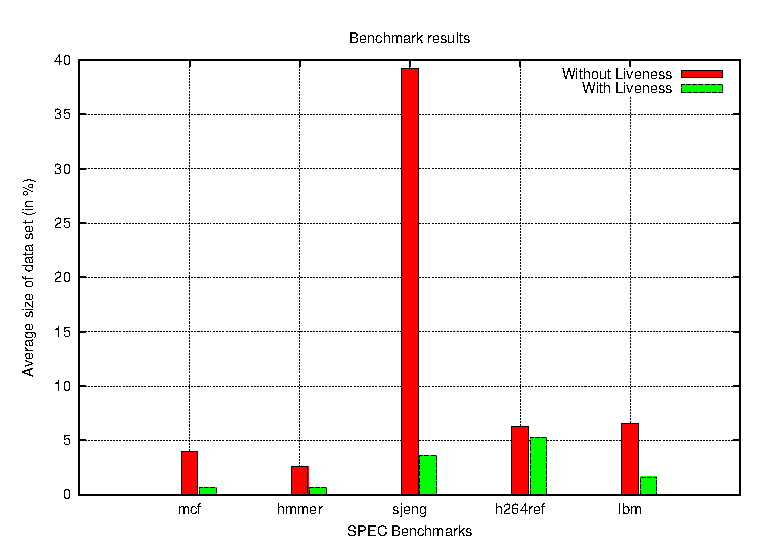
\includegraphics[width=0.8\textwidth]{graph.eps}
\caption{Percentage reduction in size of data set for Reaching definition analysis with and without liveness}
\label{fig:bench_mark}
\end{figure}

\section{Summary}
We have implemented a query for reaching definition analysis with and without liveness using PRISM. Other queries which are 
implemented using PRISM are Liveness analysis, Strongly Liveness analysis, Liveness analysis with aliasing
and Strong liveness analysis with aliasing. 

In order to compare the performance between reaching definition analysis with and without liveness, we tested both for SPEC Benchmarks.
For each query we measured the average size of the set at each program point. In general, we observe that anerage size of the set at each program 
point in liveness-based analysis is much smaller then that of the normal reaching definition analysis.



%%%%%%%%%%%%%%%%%%%%%%%%%%%%%%%%%%%%%%%%%%%%%%%%%%%%%%%%%%%%%%%%%%%%%%%%%%%%%
\chapter{Future Work}
 
This report describes the method of doing incremental analysis in bit-vector framework. This method performs incremental analysis for a single change in a program
but in general multiple changes are also possible, so we need a method which can also perform incremental analsis for multiple changes.
It also describes some issues in doing incremental analysis in Constant propagation. In Consant propagation we need to create affected region for almost all the cases.
We may restrict the size of the affected region even if we cannot avoid it. We need some method so that we can restrict the size of the affected region which will be one 
of our future work.

Current PRISM framework supports context sensitive bi-directional analysis. Incremental analysis is not yet implemented in current framework. As a part
of first stage of the project, queries for both reaching definition analysis with and without liveness have been implemented.

The current specification does not allow the user to specify data flow variables and equations as seen in literature. It places contraints on the type of analysis 
defined. It allows those analysis which has single data flow variable. Therefore, the anlysis writer needs to convert multi-variable equation to single-variable 
equation which is an extra work done by the writer. The specifications can be extended to allow analysis containig multiple variables.





%%%%%%%%%%%%%%%%%%%%%%%%%%%%%%%%%%%%%%%%%%%%%%%%%%%%%%%%%%%%%%%%%%%%%%%%%%%%%
\appendix

\chapter{User Manual of PRISM} \label{ap:A}
This section describes setting up PRISM on ubuntu system. First section describes steps for setting up PRISM and how to generate an analyzer.
Second section describes how to analyze a program using generated analyzer.

\section{Steps for setting up PRISM on Ubuntu and generating the analyzer}

The following are the steps :
\begin{itemize}
 \item  Add all the locations of jar files to classpath by setting the environment variable \textbf{CLASSPATH}. 
 \item Create an environment variable PRISMROOT and store it in the url of PRISM root directory
 \item Create a directory inside \$PRISMROOT/darpan directory and name the directory as the name of the package defined in kulang 
 files. Copy all the specification files.
 \item Run the script \textbf{populatemodel.sh}. This will create a signature of the analysis.
 \item Update `\textbf{.ini}' file.
	\begin{itemize}
	 \item \$\textbf{PRISMROOT} : location of PRISM root directory.
	 \item \$\textbf{PRISMMODEL} : location of the signature file i.e.\textbf{Lpum.cdf}
	 \item \$\textbf{REPOSDIR} : location where test result should be dumped
	 \item \$\textbf{RREPOSDIR} : location from where IR should be read
	\end{itemize}
\item Update  \textbf{.prj} file and set the path of a program to be analyzed
\item Compile all the kulang files using command `\textbf{runKulangC filename}'. After successfull compilation, `\textbf{.java}' 
 files will be created and, the generated analyzer would be created and compiled in the same directory.
\end{itemize}

\section{Running an analysis in PRISM}
Following are the steps to run an analysis in PRISM.
\begin{itemize}
 \item Write a program to be analyzed.
 \item Compile the program by using following command:
 
 \textbf{./cppfe --edg--gcc -O `location\_of\_IR' `filename' }
 
 location of IR should be same as the location present in \$\textbf{IRREPOSDIR}. For more options of cppfe, use the argument 
 `\textbf{--help}'.
 
 \item Go to the analysis directory and update `\textbf{runPrism.sh}' file. 
 \item Run the script `runPrism.sh' script. The results will be dumped into the director \$\textbf{REPOSDIR} as specified in `.ini' file
 \end{itemize}

\section{Steps for setting up PRISM in eclipse}
\begin{itemize}
 \item Open eclipse, create a new project and import the Driver and Client files of the analysis in the project.
 \item Go to project properties–build path–add external jar. Add all the jar files present in \textbf{\$PRISMROOT/lib}.
 \item Go to run configurations and create a new run configuration. In the VM arguments section, create an argument -DENVFILE=’path of .ini
file’ In the program arguments give first argument the path of .prj file and second argument the location where test results are to be dumped.
\item Write a c program to be analyzer. The name of the front end compiler to be used is cppfe. Compile the file using the command cppfe ’file-name’.
Also give the argument –edg–gcc and -O followed by location where IR should be generated. It should be the same as location of \textbf{\$IRREPOSDIR} given in
previous section.
\item Go to eclipse and run the Driver file using the run configuration created in the previous section.
\item The results will be dumped into the director \$\textbf{REPOSDIR} as specified in `.ini' file
\end{itemize}

 
 
 
 
 
\chapter{PRISM APIs}\label{ap:B}

This section describes the APIs that we have used in our implementation. An exhaustive list appears in PRISM documentation.

\section{API to access IR}
\texttt{Expr} is the base class that represents the expression in IR. This class has sub classes to represent the type of expressions, such as Unary, Binary etc.
Following are some of the API to excess the expression in IR :
\begin{itemize}
 \item \texttt{getCorrNE(Set st)}: This function takes the pointer information at the program point as a parameter and returns a set of variables that an expression represents.
 
 For e.g. If \texttt{*b} is an expression and \texttt{\{b$\rightarrow$ a, b$\rightarrow c$\}} is a pointer information, then function will return \{a,c\}
 
 \item \texttt{RvalNE(boolean lr, Set aliasSet, Set copySet)} : This function takes pointer information as a parameter and returns a set of variables used in an expression
 
 For e.g. If \texttt{*b} is an expression and \texttt{\{b$\rightarrow$ a, b$\rightarrow$c\}} is a pointer information, then function will return \{a,b,c\}
 
 \item \texttt{pointsTo(Set st)} : This function takes a set of pointer information as a parameter and returns pointees of that expression
 \item \texttt{operands()} : returns the operands used in the expression
 \item \texttt{operator()} : returns operators used in the expression
 \item \texttt{lineNum()} : returns line number of the expression
 \item \texttt{NE()} : returns the NamedEntities of the operands in the expression
\end{itemize}

\section{APIs to find properties of NamedEntity}
\begin{itemize}
 \item \texttt{coveredBy(NamedEntity ne, boolean must)} : it returns whether a given namedEntity is may or must covered by the passed namedEntity.
 
 For e.g. a.b is covered by a
 \item \texttt{getDataType()} : returns the data type of the operand

 \item \texttt{isGlobal()} : returns true if the given namedEntity is global
 \item \texttt{getNEsFromReturn(Expr ex)} : returns the namedEntity of the variables used in the return statement
 \item \texttt{getNEsFromCall(Expr ex)} : returns the namedEntity of the variables used in the call statements
\end{itemize}


\chapter{Specifications of developed kulang queries}\label{ap:C}
\section{Intra-procedural Reaching definition analysis}
Following is the specification for Intra-procedural reaching definition analysis.

\begin{lstlisting}
//Package declaration
package darpan.klgLib;

//Typedef
tup :: tuple(int,NamedEntity),
res :: set tup;

//Use declaration
fn_use darpan.klgLib;
fn_decl
res Meet (res, res),
res cartProduct ( set NamedEntity, set NamedEntity);

java_use darpan.klgLib.Aux;
java_decl
int line(Expr),
set tup HasElement(NamedEntity,res),
set NamedEntity IRefValNE@darpan.solverlib.FLAAnalysis(Expr,
					  boolean,IRObject),
set NamedEntity getNEs(Expr),
set NamedEntity getNEsFromCall(Expr),
set NamedEntity getNEsFromReturn(ASTnode),
boolean isLive(Expr,set NamedEntity),
set NamedEntity aliasClosure ( Expr, IRObject),
boolean printSet(set NamedEntity),
boolean isDref(Expr),
boolean isMust(set NamedEntity),
set NamedEntity getPtsto(res,Expr),
res getPointesOf(res,set NamedEntity),
set NamedEntity dref(res,Expr),
set NamedEntity getLhsSet(res,Expr),
NamedEntity getKillCandidate(set NamedEntity),
NamedEntity getIllegalNE();

//Mode
[FLA];

//Declaration of lattice type
lattice L ::  res; 

lCreaches_FG implements lCreaches_FG:

//Declaration of top value
top : (res){};

//Declaration of meet function
A meet B : A+B;

//Declaration of boundary value
BoundaryValue :(res){} ;

//Specifications of flow function for various statements
ForwardNodeflow( n: Symbol_AST, S: L )
	let
		ne=NE(n);
		exp=initExpr(n);
		line_no=line(exp);
		kill=HasElement(ne,S);
		def={[line_no,ne]};
	in
		(S-kill)+def;

ForwardNodeflow( n: Binary, S: L ) 
	if(operator(n)=='=')
	then
		let
			ne=NE(n);
			l_exp=lhs(n);
			l_var=getNEs(l_exp);
			line_no=line(l_exp);
			kill=HasElement(ne,S); 
			def={[line_no,ne]};
		in
			(S-kill)+def
	else
		S
	endif;


ForwardNodeflow( n: Unary, S: L )
	let
		ne=NE(n);
		line_no=line(n);
		kill=HasElement(ne,S);
		def={[line_no,ne]};
	in
		(S-kill)+def;

ForwardNodeflow( n: Call, S: L ) 
	S;

ForwardNodeflow( n: _, S: L ) 
	S;

ForwardEdgeflow(E: _, S: L) 
	S;
\end{lstlisting}


\section{Liveness-based Intra-procedural Reaching definition analysis}
Following is the specification for Liveness-based Intra-procedural Reaching definition analysis.
\begin{lstlisting}
//Package declaration
package darpan.klgLib;

//Typedef
tup :: tuple(int,NamedEntity),
livenesslattice :: set NamedEntity,
res :: set tup;

//Use declaration
fn_use darpan.klgLib;
fn_decl
res Meet (res, res),
res cartProduct ( set NamedEntity, set NamedEntity);

java_use darpan.klgLib.Aux;

java_decl
int print_set(set NamedEntity),
res removeNonLive(res,livenesslattice),
int line(Expr),
set tup HasElement(NamedEntity,res),
set NamedEntity IRefValNE@darpan.solverlib.FLAAnalysis(Expr,
					  boolean,IRObject),
livenesslattice getNE(Expr),
livenesslattice getNEs(Expr),
set NamedEntity getNEsFromCall(Expr),
set NamedEntity getNEsFromReturn(ASTnode),
boolean isLive(Expr,set NamedEntity),
boolean Check_datatype_call(Expr),
set NamedEntity aliasClosure ( Expr, IRObject),
livenesslattice useInRhs(res,Expr),
boolean printSet(set NamedEntity),
boolean CHECK(Expr),
boolean check_datatype(Expr),
boolean check_datatype_lhs(Expr),
boolean isDref(Expr),
boolean isMust(set NamedEntity),
set NamedEntity getPtsto(res,Expr),
res getPointesOf(res,set NamedEntity),
set NamedEntity dref(res,Expr),
set NamedEntity getLhsSet(res,Expr),
NamedEntity getKillCandidate(set NamedEntity),
set NamedEntity emptySet(),
NamedEntity getIllegalNE();

//Mode
[FLA];

//Declaration of lattice types
Forwardlattice Rec ::  res;
Backwardlattice Liv :: livenesslattice;

lCreaches_FG implements lCreaches_FG:

//Declaration of types of forward and backward lattices
ForwardTop : (res){};
BackwardTop : (livenesslattice){};

//Declaration of meet functions
A ForwardMeet B : Meet(A,B);
A BackwardMeet B : A+B;

// Specification of boundry values
ForwardBoundaryValue : (res){};
BackwardBoundaryValue :(livenesslattice){} ;

// Specification of backward flow functions for various statement types
BackwardNodeflow( n: Binary, R: Rec, L:Liv )
if(check_datatype_lhs(lhs(n))==true && 
		      check_datatype(rhs(n))==true)
then
        let
                rt_expr=rhs(n);
                check =CHECK(n);
                lt_expr=lhs(n);
                rone=getNEs(rt_expr);
		lone=getNEs(lt_expr);
                x = if(operator(n)=='=')
                    then
                            if(isLive(lt_expr,L)==true)
                            then
                                 (L - lone) + rone
                            else
                                  L
                            endif
                   else
                                (L + lone) + rone
                   endif;
        in
                x
else
        L
endif;

BackwardNodeflow( n: Unary,R: Rec, L:Liv )
if(check_datatype(n)==true)
then
        let
             operands_ne=getNEs(n);
        in
             L+operands_ne
else
        L
endif;

BackwardNodeflow( n: Call, R: Rec, L:Liv )
if(Check_datatype_call(n)==true)
then
        let
             d = emptySet();
             UseInCall = getNEsFromCall(n);

        in
             d + L + UseInCall

else
        L
endif;

BackwardNodeflow( n: _,R: Rec, L:Liv)
        L;


BackwardEdgeflow(E: _,R: Rec, L:Liv)
        L;



ForwardNodeflow( n: Symbol_AST,R: Rec,L:Liv)
if(check_datatype(initExpr(n))==true)
then
        let
                ne=NE(n);
                exp=initExpr(n);
                check =CHECK(exp);
                line_no=line(exp);
                kill=HasElement(ne,R);
                def={[line_no,ne]};
                sur=(R-kill)+def;
                survive=removeNonLive(sur,L);
        in
                survive
else
        R
endif;



ForwardNodeflow(n: Binary,R: Rec,L:Liv)
if(check_datatype_lhs(lhs(n))==true && 
		      check_datatype(rhs(n))==true)
then
        let
                check =CHECK(n);
                rt_expr=rhs(n);
                l_exp=lhs(n);
                ne=NE(n);
                line_no=line(l_exp);
                kill=HasElement(ne,R); 
                def={[line_no,ne]};
                sur=(R-kill)+def;
                survive=if(operator(n)=='=')
                        then
                               removeNonLive(sur,L)
                        else
                               removeNonLive(R,L)

                        endif;
        in
                survive
else
        S
endif;





ForwardNodeflow( n: Unary,R: Rec,L:Liv)
if(check_datatype(n)==true)
then
        let
                check =CHECK(n);
                ne=NE(n);
                line_no=line(n);
                kill=HasElement(ne,R);
                def={[line_no,ne]};
                sur=(R-kill)+def;
                survive=removeNonLive(sur,L);
        in
                survive
else
        R
endif;

ForwardNodeflow( n: _,R: Rec,L:Liv)
        let
                survive=removeNonLive(R,L);
        in
                survive;

ForwardEdgeflow(E: _,R: Rec,L:Liv)
        let
                survive=removeNonLive(R,L);
        in
                survive;

Function res Meet ( A: res, B: res)
let
        diff=A+B;

in
        diff;

                                                                                                           


\end{lstlisting}


\renewcommand{\bibname}{References}
\begin{small}
\bibliography{report1}
\bibliographystyle{plain}
\end{small}





\end{document}
